\documentclass[output=paper]{langsci/langscibook} 
\author{Jonathon Lum \affiliation{University of Melbourne}} 

\markuptitle{An egophoric analysis of Dhivehi verbal morphology}{An egophoric analysis of Dhivehi verbal morphology}
%\shorttitlerunninghead{}

% \title{\texorpdfstring{Word formation and word history:\\ The case of
%  \textsc{capitalist} and \textsc{capitalism}}{Word formation and word
% history:  CAPITALIST and
% CAPITALISM}}

% \renewcommand{\lsCollectionPaperFooterTitle}{Word formation and word
% history: The case of  \noexpand\textsc{capitalist} and
% \noexpand\textsc{capitalism}}

 
\abstract{Egophoricity is a typologically rare category in which first-person statements and second-person questions share the same marking (“egophoric”), while other contexts generally lack this marking. This chapter presents evidence that certain verbal suffixes in Dhivehi (Indo-Aryan, Maldives) mostly show an egophoric distribution, contrary to previous analyses of these suffixes as first/second person markers. Dhivehi is thus the first Indo-European language reported to show an egophoric pattern. Aside from the distribution of the relevant suffixes in first-person statements and second-person questions, further evidence for an egophoric analysis may be found in contexts where a third-person nominal subject refers to the speaker or addressee ‒ in these contexts the appearance of the relevant suffixes is more consistent with egophoricity than person marking. However, egophoricity in Dhivehi is restricted to finite, volitional stems in certain tenses/aspects/moods, and some relics of an older person-marking system survive. Finally, it is proposed that egophoricity in Dhivehi may have developed from a reanalysis of person markers in reported speech, in a process similar to that described by \cite{WidmerZemp2017} for certain Tibeto-Burman languages.
}

\begin{document}
\maketitle

\section{Introduction}\label{s:jl1}

\subsection{Background and outline}\label{s:jl1-1}

In Dhivehi, the Indo-Aryan language of the Maldives, finite volitional-stem verbs in some tenses/aspects/moods are seemingly marked for person, though different linguists have listed different forms for certain parts of the verbal paradigm. This is true especially for the second person, which has been grouped both with the first person (\citealt[23--27]{CainGair2000}) and partly with the third person (\citealt[166--169]{Fritz2002}). This chapter offers a new analysis of the situation, presenting data from recent fieldwork as well as from written material to argue that Dhivehi in fact displays an egophoric or “conjunct-disjunct” pattern of verbal marking. Egophoricity is a typologically rare pattern in which verbs in second-person questions are marked like verbs in first-person statements, while verbs in second-person statements are marked like verbs in third-person questions/statements (e.g., \citealt{Hale1980}; \citealt{Creissels2008}; \citealt{SanRoque2018}). The presence of this pattern in Dhivehi may partly explain the inconsistencies between some existing descriptions of the language, given that verbs with second-person subjects may resemble verbs with either first- or third-person subjects, depending on the sentence type.

More importantly, the existence of egophoricity in Dhivehi is of considerable typological significance, as grammatical systems of this kind are highly unusual cross-linguistically, and have never before been reported for an Indo-European language. The origins of egophoricity in Dhivehi are therefore of some interest, especially given the isolation of the Maldives from regions (such as the Tibeto-Burman area) where egophoricity has previously been reported. The details of egophoric systems vary greatly (\citealt{Floydetal2018}), and the Dhivehi system shows some features that have not been (widely) reported on before, and which may shed light on egophoricity as a cross-linguistic phenomenon. These include the use of egophoric marking in first-person questions, and an interaction with a tendency (motivated by politeness) towards third-person nominal reference in place of first- and second-person pronouns in many contexts.

Like many other languages with egophoricity, Dhivehi also has a reported speech construction in which egophoric markers may be seen as showing co-reference between the subject of the matrix clause and the subject of the embedded clause, while egophoric marking is absent when these subjects are not co-referential. And like in many other egophoric systems, Dhivehi egophoric markers are restricted to volitional contexts, though the existence of separate “involitive” morphology means that the alternation between egophoric and alterphoric marking of the same stem is never deployed to show contrasts in volition, unlike in some other languages (e.g., the Tibeto-Burman language Newar, \citealt{Hale1980}).\footnote{See §‎\ref{s:jl1-3} for definitions of the terms \textit{egophoric} and \textit{alterphoric}.} It is therefore hoped that this chapter will be of interest both to scholars of Dhivehi and to scholars working on egophoricity and related areas such as volitionality, person marking, and reported speech.

This chapter is divided into six main sections. The current section introduces the prospect of an egophoric analysis for Dhivehi and the significance of such an analysis, provides a brief profile of the language, its speakers and dialects, and also makes some brief notes on terminology and data collection. §‎\ref{s:jl2} provides a summary of some previous accounts of person marking in Dhivehi, highlighting their inconsistencies. §‎\ref{s:jl3} introduces some issues with those accounts and shows how an egophoric analysis is a better fit for the data, presenting evidence from second-person statements as well as from contexts where speakers use third-person nominal reference in place of first- or second-person pronouns. Data from reported speech are also shown to be consistent with this analysis. However, elements of an older person-marking system appear to be present in the context of first-person questions and in the distribution of the archaic/literary suffix ‑\textit{mu}. §\ref{s:jl4} discusses person marking in some of Dhivehi’s conservative southern dialects, and suggests a possible way in which egophoricity could have developed in the northern dialects (including the standard Malé dialect). In particular, I propose that (northern) Dhivehi may have undergone a similar process to that described by \cite{WidmerZemp2017}, in which a person-marking system is gradually reanalyzed and reshaped into an egophoric system, via a semi-direct speech construction. Finally, §‎\ref{s:jl5} summarizes the chapter and suggests some areas for future research.


\subsection{Dhivehi}\label{s:jl1-2}

Dhivehi (or “Maldivian”) is an Indo-Aryan language spoken throughout the Maldives, where it is the national language. Dhivehi has more than 340,500 speakers (\citealt{Lewis2014}), mostly in the Maldives but also in smaller numbers abroad. A dialect of the language (sometimes known as Mahl) is spoken on Minicoy, an island belonging to the Indian union territory of Lakshadweep, to the north of the Maldives. Despite the increasing encroachment of English, Dhivehi continues to enjoy a dominant status in the Maldives, where it is the main language of communication in mass media, government, and home life. 

There are two main dialect groups (see Figure \ref{fig:jl1}, below): a northern group spanning from Minicoy all the way to Laamu Atoll, and a southern group comprising the dialects of Huvadhu, Fuvahmulah, and Addu. At the heart of the northern dialect group is the standard dialect based on the language of Malé. This standard variety is used throughout the country in mass media and in official contexts, and is understood all across the archipelago. The atolls nearest to Malé use this dialect with only some slight variants, while more far-flung islands or atolls (such as Minicoy and Laamu) have dialects that are related but more clearly distinct.\footnote{The northern dialect group is probably not as homogeneous as has sometimes been claimed (e.g., \citealt[13]{Fritz2002}). According to the consultants from Malé and Laamu with whom I worked during field trips in 2013‒2015, as well as some expatriates in Australia, Malé speakers can barely understand the Laamu dialect, if at all. They also report that some northern islands such as Naifaru (in Lhaviyani Atoll), have very distinct dialects too. More work is needed on this subject. Nonetheless, it does appear to be true that the northern dialect group is more homogeneous than the southern dialect group.} 

The dialects in the southern group are the most conservative and show similarities with older varieties of Sinhala, the language to which Dhivehi is most closely related.\footnote{According to \cite{Cain2000}, Dhivehi and Sinhala may have begun to diverge as early as the 3$^{rd}$‒1$^{st}$ centuries BCE, but were in contact for many centuries after that.}
The Addu and Fuvahmulah dialects are described by \cite{Fritz2002}, though the Huvadhu dialect is practically undocumented (except for a small amount of information in \citealt{Maumoon2002} and \citealt{Wijesundera1988}). These dialects are not understood by Malé speakers (though as indicated earlier, southerners can understand the Malé dialect due to exposure), and are apparently not mutually intelligible with each other either.

\begin{figure}
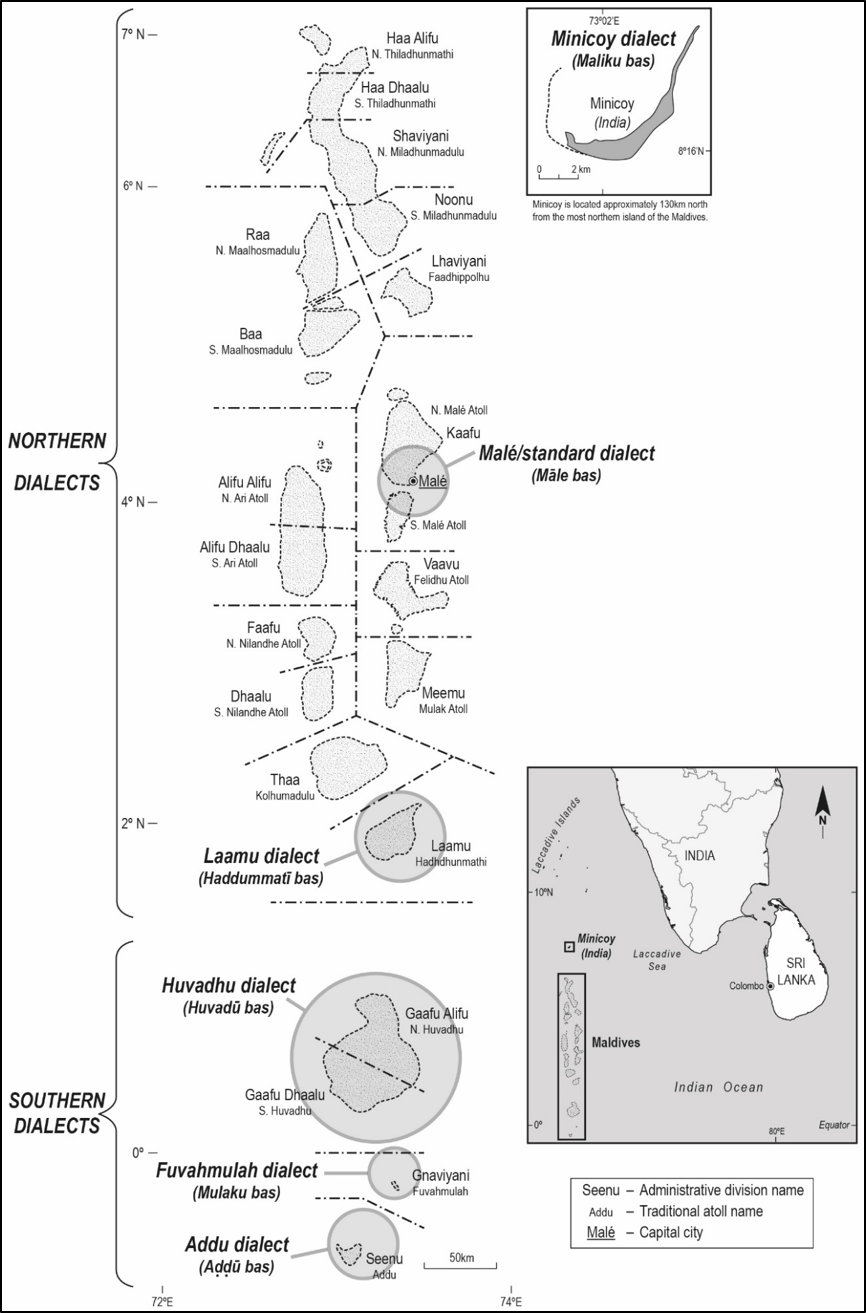
\includegraphics[width=\textwidth]{figures/lum-1.png}
\caption{Dialect Map of Maldives}
\label{fig:jl1}
\end{figure}


 Even the standard/Malé dialect has attracted little scholarly attention, in part because the Maldives has been relatively inaccessible to outsiders until the late 20$^{th}$ century, and in part because the language has sometimes been assumed to be very similar to Sinhala. Thus, although the first word lists date back to the 17$^{th}$ century (\citealt{Pyrard1619}) and the first grammatical sketches to the early 20$^{th}$ century (\citealt{Geiger1919}), comprehensive dictionaries and grammatical descriptions were not made until the last few decades. At present, the best Dhivehi-English dictionary is \cite{Reynolds2003}, and the most detailed grammars are \cite{Wijesundera1988}, \cite{Cain2000} (also re-worked into a sketch grammar, \citealt{CainGair2000}, \cite{Fritz2002}, and especially \cite{Gnanadesikan2017}. There are also a number of Dhivehi-medium works on the language, housed in various educational and research institutions in the Maldives. Most of these are prescriptive (e.g., \citealt{Ahmad1970}; \citealt{Saudiq2012}).

As is the case for Sinhala, there is evidence of substantial historical contact between Dhivehi and Dravidian languages (\citealt{Cain2000}), and in later periods Dhivehi has also come into contact with Arabic, Portuguese and English. Typologically, Dhivehi has much in common with Sinhala (spoken in Sri Lanka) and other languages of the South Asia region. Dhivehi has a predominant SOV word order, and noun phrases are consistently head-final. The language makes considerable use of clause chaining, with sentences made up of only one finite clause preceded by any number of non-finite medial clauses. Pro-drop is typical especially in spoken language, and clauses tend to omit as many arguments as can be retrieved from context. For reasons that are not entirely clear (but probably due in part to language contact), Dhivehi has lost much of the morphological complexity found in Sanskrit and the Prakrits from which it descends. Gender is not a category in the standard language (even in pronouns), and number is not obligatorily marked except on nouns denoting humans. There is no morphological distinction between the nominative and accusative (both falling under an unmarked “direct” case), though the standard language does also have separate dative, locative, genitive, instrumental/ablative, comitative and vocative cases. In terms of alignment, Dhivehi therefore shows “neutral” alignment in its nominal and pronominal morphology (i.e., core arguments are never distinguished from each other morphologically).

Verb paradigms vary according to stem type, with slightly different patterns for monosyllabic stems (e.g., \textit{ka-nī} ‘eating’), polysyllabic \textit{a}-stems (e.g., \textit{jaha-nī} ‘striking’), polysyllabic \textit{nn}-stems (e.g., \textit{ganna-nī} ‘buying’), \textit{e}-stems including inactive/intransitive/involitive verbs (e.g., \textit{e$^n$ge-nī} ‘knowing’), and irregular verbs (\citealt[22--25]{CainGair2000}; \citealt[136--146]{Gnanadesikan2017}). For all stem types, a number of tenses, aspects and moods may be distinguished morphologically. Verbs in the present, simple past, simple future, perfect, potential/optative, and irrealis/conditional are generally considered to carry person marking (e.g., \citealt[23--27]{CainGair2000}; \citealt[Chapter 8]{Gnanadesikan2017}), though in this chapter I will argue that this is in fact egophoric marking. In contrast, verbs with progressive aspect simply take the suffix ‑\textit{(n)ī} regardless of person or number. The same suffix is also used as a focus marker, attaching to verbs that appear in non-canonical (i.e., non-final) position regardless of person, number, or aspect (this “focus marking”, along with the unusual word order and various prosodic cues, puts pragmatic focus on whatever constituent follows the verb). Progressive/focus verb forms are very common in the language and appear in many contexts where English or other languages would use a conjugated verb. 

Like Sinhala, Dhivehi has an alternation between active, volitional verbal morphology and inactive/intransitive/involitive morphology (which \citealt{CainGair2000} usefully refer to as \textsc{in}-morphology), with \textsc{in}-verbs never carrying person marking. This morphological category interacts with various syntactic constructions and plays an important role in the grammar of the language. \textsc{in}-verbs are used in many intransitive clauses, passive (or at least, “inactive”) clauses, as well as in clauses where the agent acts accidentally or against his own will. In addition, \textsc{in}-verbs may be used to show politeness, abilities, or counter-expectations of the speaker, among other functions (see \citealt{Cain1995}; \citealt[56--60]{CainGair2000}; \citealt[248--257]{Gnanadesikan2017}).

Along with progressive/focus verb forms, Dhivehi makes much use of various other verb forms and verbal nouns that do not show person marking. In particular, converbs are used in clause chains, and participles in adverbial clauses, complement clauses, and relative clauses. In fact, as \cite[289]{Gnanadesikan2017} notes, in general Dhivehi allows at most one finite verb per sentence. It should also be noted that there are no copular verbs in the language ‒ statements of equivalence are made by attaching a copular marker directly to the subject noun phrase (see \citealt[236--237]{Gnanadesikan2017}). The prevalence of progressive/focus verb forms, \textsc{in}-verb forms, converbs and participles (and other non-finite verbs), in conjunction with the lack of copular verbs, means that there are relatively few verbs in ordinary Dhivehi discourse that show any kind of person marking, a point to which I return in §\ref{s:jl1-4}.



\subsection{Terminological note}\label{s:jl1-3}

In this chapter I use the terms \textit{egophoric} and \textit{alterphoric}, following \cite{Post2013}. The term \textit{egophoric} (from \citealt{Tournadre1992}; \citeyear{Tournadre1994}) has become fairly well established in recent years (e.g., \citealt{Floydetal2018}), displacing earlier terms such as \textit{conjunct} (\citealt{Hale1980}). Egophoric markers are used in first-person statements and second-person questions, though they sometimes appear elsewhere in some languages. Verbal marking that appears only in other contexts, especially third-person statements/questions and second-person statements, was originally labelled \textit{disjunct} marking by \citeauthor{Hale1980}, though other terms such as \textit{non-egophoric} have more recently become popular. Instead of \textit{non-egophoric}, I use the term \textit{alterphoric} as a convenient way of referring specifically to non-egophoric marking on finite, volitional-stem verbs in the relevant tenses/aspects/moods, i.e., the same stems which may carry egophoric marking. The term \textit{non-egophoric} is less suited to this purpose because it tends to imply ‘not egophoric’, yet in Dhivehi, non-finite verbs (including converbs, participles, and infinitives), \textsc{in}-verbs, and verbs in the progressive/focus form are unable to carry either egophoric or alterphoric marking, but in a general sense are non-egophoric (i.e., not egophoric) too. This will become clearer throughout this chapter. For recent overviews of terminology used in the egophoricity literature, see \cite[6--9]{SanRoque2018} and \cite[35]{WidmerZemp2017}.

\subsection{Data sources}\label{s:jl1-4}

The data presented in this chapter mostly come from elicitation sessions conducted with a 34-year-old native Dhivehi speaker in Fonadhoo, Laamu Atoll during fieldwork in 2014‒2015. This speaker is fluent in both the Laamu and Malé dialects, and provided judgements and example sentences for both dialects. These judgements and sentences were subsequently verified separately with more than twenty other native speakers in Laamu, Malé, and in Australia (where some native speakers reside for work or study). 
   To supplement the elicited data, a number of online searches for written language examples were conducted with the assistance of another native speaker consultant. Literacy rates are extremely high in the Maldives, and recent years have seen a rapid growth in Dhivehi language material online, including news, social media, blogs, and collections of short stories. Much of this material is written in Thaana, a right-to-left script unique to Dhivehi. Using a search engine, searches were made using combinations of common subjects (e.g., pronouns and kin terms) with common verbs (e.g., \textit{kuranī} ‘doing’) in their volitional form and in the appropriate tenses/aspects/moods for the grammatical contexts at issue. The examples obtained by this process all come from short stories published online, on various websites and by various authors. Where necessary, more context is provided with each example. 

   Finally, a few written language examples from her corpus of Dhivehi online news stories were kindly shared by Amalia Gnanadesikan (personal communication), and some other examples are sourced from existing descriptions of the language such as \cite{CainGair2000} and \cite{Gnanadesikan2017}. 

   The use of these data sources was necessitated by the nature of the research question, which relates to verbal marking in a range of grammatical contexts. Some of these contexts, such as second-person statements and first-person questions, are relatively rare and may not necessarily appear in a corpus of spoken language texts.\footnote{The corpus of spoken texts I collected during my fieldwork in the Maldives, for example, did not contain clear examples of finite, volitional-stem verbs in the grammatical contexts at issue. This corpus, which was compiled for a separate project on spatial language and cognition (see \citealt{Lum2018}; \citealt{Palmer2017SIP}; \citealt{Palmer2017Typ}), mostly included recordings of speakers engaged in description tasks and instructional texts, with some narratives.} 
   This problem is common in studies on egophoricity, and unsurprisingly much of the literature going back to \cite{Hale1980} relies at least in part on elicited data. It should also be noted that for Dhivehi in particular, it is not easy to find in naturally occurring texts the relevant data points to decide between a person-marking analysis and an egophoric analysis. Aside from the fact that the right contexts (e.g., second-person statements) are somewhat rare anyway, egophoric/alterphoric marking (or person marking according to previous analyses) in Dhivehi occurs only on finite, volitional-stem verbs that are not in the progressive/focus form. This means that the appearance of \textsc{in}-verbs (which are required in inactive/intransitive/involitive sentences, as mentioned in §\ref{s:jl1-2}) does not help to decide between analyses, nor does the appearance of non-finite or progressive/focus forms. As discussed in §\ref{s:jl1-2}, these verb forms are extremely common in Dhivehi. The use of direct elicitation and the World Wide Web therefore facilitated easier access to verb forms and grammatical contexts that are relatively uncommon in ordinary discourse.

\section{Previous accounts of person marking in Dhivehi}\label{s:jl2}

Descriptions of person marking in (standard) Dhivehi are provided by \cite{Geiger1919}, \cite{Wijesundera1988}, \cite{Cain2000}, \cite{Fritz2002}, and most recently \cite{Gnanadesikan2017}. A few other works (\citealt{CainGair2000}; \citealt{Maumoon2002}) contain descriptions of person marking based on \cite{Cain2000}. In addition, there are some prescriptive works (in Dhivehi language) that offer guidelines on person marking (e.g., \citealt{Ahmad1970}; \citealt{Saudiq2012}). However, many of these various accounts disagree on aspects of the Dhivehi person-marking system.  In particular, they mostly agree on third-person forms, but not on first- and second-person forms. \citeauthor{Geiger1919}’s (\citeyear{Geiger1919}) description contains some clues as to how the system worked in the early 20$^{th}$ century (see §‎\ref{s:jl4-3}), but unfortunately appears to confuse different tenses and aspects throughout paradigms. \cite{Wijesundera1988} describe first-person and third-person forms, but not the second person. I will therefore concentrate on the more recent descriptions provided by \cite{CainGair2000} and \cite{Fritz2002}, with some mention also of the prescriptive literature. The most recent description of the language, \cite{Gnanadesikan2017}, analyses the relevant markers as person markers, but like \citeauthor{Wijesundera1988}, describes them as first-person and third-person markers. Referencing an earlier version of the current chapter, \cite[138]{Gnanadesikan2017} acknowledges that second-person forms are variable, and accepts that at least some speakers show a split, with second-person subjects in statements triggering the same verbal agreement as third-person subjects, but in questions the same verbal agreement as first-person subjects.

\subsection{Fritz’s (2002) account}\label{s:jl2-1}

According to \cite[166]{Fritz2002}, “[t]he finite verb is characterized by a three person system distinguishing singular and plural”. For the simple present tense of polysyllabic a-stem verbs in the Malé dialect, she gives the paradigm outlined in Table \ref{tab:jl1} below:\footnote{ In this table and elsewhere, -\textit{V}: indicates lengthening of the final vowel in the stem.}

\begin{table}
\begin{tabularx}{\textwidth}{lll}
\hline
\textbf{Person/number} & \textbf{Suffix} & \textbf{Example from \textit{balanī} ‘looking’ (stem: \textit{bala}-)}\\
\hline
\textsc{	1sg	}	&	\textit{	-n	}	&	\textit{	bala-n	}	\\
\textsc{	2sg	}	&	\textit{	-V:	}	&	\textit{	balā	}	\\
\textsc{	3sg	}	&	\textit{	-V:	}	&	\textit{	balā	}	\\
\textsc{	1pl	}	&	\textit{	-mu / -n	}	&	\textit{	bala-mu / bala-n	}	\\
\textsc{	2pl	}	&	\textit{	-mu / -V:	}	&	\textit{	bala-mu / balā	}	\\
\textsc{	3pl	}	&	\textit{	-V:	}	&	\textit{	balā	}	\\
\hline
\end{tabularx}
\caption{Person marking on simple present tense polysyllabic a-stem verbs according to \cite[168--169]{Fritz2002}}
\label{tab:jl1}
\end{table}

Fritz thus presents a simple first- versus non-first-person distinction in the singular, but a more complicated picture in the plural. She states that -\textit{mu} is used as a first/second-person plural marker, and lists this in her own tables. However, she notes in her prose that -\textit{n} is an alternative to -\textit{mu} in the first-person plural, and -\textit{V}: may be used in the second-person plural, both of which she interprets as analogical formations based on the equivalent singular forms. The third person is simply -\textit{V}: in both singular and plural. 

   For the simple past (in her terms “finite preterite”), which has a different stem, \cite[174--176]{Fritz2002} describes the same basic pattern for person agreement: a first- versus second/third-person dichotomy in the singular, but a first/second- versus third-person dichotomy in the plural, with the third person having the same form (-\textit{Ø}) in both singular and plural. She does not specify whether the first- and second-person plural also have alternative forms identical to their singular equivalents as they do in the present tense. Additionally, she regards the perfect as a compound of the “absolutive” (converb) form of the main verb followed by the simple past of the now obsolete verb *\textit{fianī} ‘put’ (\citealt[225--226]{Fritz2002}) ‒ thus, the perfect follows the same person-marking template as the simple past. However, for the simple future (which also has its own stem), \cite[176‒178]{Fritz2002} presents a first- versus second/third-person distinction that is not sensitive to number. She also gives an alternative, archaic form -\textit{ū} for the first/second-person plural, which she reports is mostly confined to literary usage. These various paradigms are summarized in Table \ref{tab:jl2} below:
   
\begin{table}
\begin{tabularx}{\textwidth}{lllll}
\hline
\textbf{Person/number} & \textbf{Simple present} & \textbf{Simple past} & \textbf{Perfect} & \textbf{Simple future}\\
\hline
\textsc{	1sg	}	&	\textit{	-n	}	&	\textit{	-n	}	&	\textit{	-fin	}	&	\textit{	-an	}	\\
\textsc{	2sg	}	&	\textit{	-V:	}	&	\textit{	-Ø	}	&	\textit{	-fi	}	&	\textit{	-e	}	\\
\textsc{	3sg	}	&	\textit{	-V:	}	&	\textit{	-Ø	}	&	\textit{	-fi	}	&	\textit{	-e	}	\\
\textsc{	1pl	}	&	\textit{	-mu / -n	}	&	\textit{	-mu	}	&	\textit{	-fimu	}	&	\textit{	-an / -ū	}	\\
\textsc{	2pl	}	&	\textit{	-mu / -V:	}	&	\textit{	-mu	}	&	\textit{	-fimu	}	&	\textit{	-e / -ū	}	\\
\textsc{	3pl	}	&	\textit{	-V:	}	&	\textit{	-Ø	}	&	\textit{	-fi	}	&	\textit{	-e	}	\\
\hline
\end{tabularx}
\caption{Person suffixes according to \cite{Fritz2002}}
\label{tab:jl2}	
\end{table}


\subsection{Cain \& Gair’s (2000) account}\label{s:jl2-2}

\cite[23--27]{CainGair2000} present a simpler picture (based on \citealt[54--63]{Cain2000}) of person marking in the contemporary standard language of Malé. According to their analysis, many tenses/aspects/moods show a distinction between an unmarked third-person form on the one hand and a “non-third” (henceforth, “first/second”) person form on the other, with no distinction between singular and plural. Tenses/aspects/moods with this marking include the simple present, simple future, simple past, perfect, irrealis, and optative. According to \citeauthor{CainGair2000}, the third person is unmarked. They report that the first/second-person marker for the simple present and simple past is -\textit{n}, but they state that the underlying form is -\textit{m}/-\textit{mu}, which appears in certain dialects and sometimes also in literary Dhivehi. Their paradigms for the simple present, simple past, perfect, and simple future are shown in Table \ref{tab:jl3} below:

\begin{table}
\begin{tabularx}{\textwidth}{lllll}
\hline
\textbf{Person/number} & \textbf{Simple present} & \textbf{Simple past} & \textbf{Perfect} & \textbf{Simple future}\\
\hline
\textsc{	1sg	}	&	\textit{	-n	}	&	\textit{	-n	}	&	\textit{	-fin	}	&	\textit{	-an	}	\\
\textsc{	2sg	}	&	\textit{	-n	}	&	\textit{	-n	}	&	\textit{	-fin	}	&	\textit{	-e	}	\\
\textsc{	3sg	}	&	\textit{	-V:	}	&	\textit{	-Ø	}	&	\textit{	-fi	}	&	\textit{	-e	}	\\
\textsc{	1pl	}	&	\textit{	-n	}	&	\textit{	-n	}	&	\textit{	-fin	}	&	\textit{	-an	}	\\
\textsc{	2pl	}	&	\textit{	-n	}	&	\textit{	-n	}	&	\textit{	-fin	}	&	\textit{	-e	}	\\
\textsc{	3pl	}	&	\textit{	-V:	}	&	\textit{	-Ø	}	&	\textit{	-fi	}	&	\textit{	-e	}	\\
\hline
\end{tabularx}
\caption{Person suffixes according to \cite{CainGair2000}}
\label{tab:jl3}	
\end{table}

\subsection{Comparison and discussion}\label{s:jl2-3}

In a review of \cite{Fritz2002}, \cite{Cain2004} criticizes \citeauthor{Fritz2002}’s account of the person-marking system, which he argues is based partly on an incorrect phonological analysis of the nasals \textit{n} and \textit{m}. According to \citeauthor{Cain2004}, both nasals neutralize to [ŋ] word-finally (rendered as <n> in writing), and the verbal endings ‑\textit{n}, -\textit{m}, and -\textit{mu} are simply allomorphs of the same suffix. The first of these appears word-finally, whereas -\textit{m} is used before a vowel, such as when followed by the sentence-final marker ‑\textit{eve} (\citealt[355]{Cain2004}). Unfortunately, \citeauthor{Cain2004} does not mention what phonetic environment attracts the -\textit{mu} form. He does, however, observe that -\textit{mu} can be used with singular subjects, which is contrary to \citeauthor{Fritz2002}’s account. \citeauthor{Cain2004} also points out that the data in \citeauthor{Fritz2002}’s text materials (\citealt[Vol. 2]{Fritz2002}) sometimes differ significantly from \citeauthor{Fritz2002}’s own description, with examples like \textit{nikumejjai-m-eve} ‘(I) went out’ (\citeyear[Vol. 2, 136]{Fritz2002}) and \textit{ahālaifī-m-eve} ‘I asked’ (\citeyear[Vol. 2, 141]{Fritz2002}), in which -m is used for the first-person singular (rather than -\textit{n}), and also examples like \textit{duśi-n ta?} ‘Have (you) seen…?’ (\citeyear[(Vol. 2) 154]{Fritz2002}) in which -\textit{n} is used for the second-person singular (rather than -\textit{Ø}). 

 Tables \ref{tab:jl4a} and \ref{tab:jl4b}\footnote{There are also some small but inconsequential differences according to stem type (e.g., \citealt[23‒27]{CainGair2000}). To simplify matters, this table is intended to represent the suffixes for polysyllabic \textit{a}-stem verbs in particular, though in most respects it is also accurate for verbs of other stem types.}
  below summarize the different accounts of person marking given by \cite{Fritz2002} and \cite{CainGair2000} (whose analysis is also followed by \citealt{Maumoon2002}) for four tenses/aspects.\footnote{The more marginal irrealis/conditional and potential/optative are not compared here as \cite{Fritz2002} does not explicitly list their forms according to person and number. No other tenses/aspects/moods are considered to have person marking.} Suffixes involving -\textit{n} (or -\textit{an} in the future) or ‑\textit{mu} (a possible allomorph or variant) are shaded in grey.
 

%%to much content in one table 
%%\begin{table}
%%\begin{tabularx}{\textwidth}{L{1.4cm}llll llllll}
%%\hline
%%\textbf{	Person/number	}	&	\multicolumn{3}{c}{\textbf{	Simple present	}}									&	\multicolumn{2}{c}{\textbf{	Simple past	}}					&	\multicolumn{2}{c}{\textbf{	Perfect	}}					&	\multicolumn{3}{c}{\textbf{	Simple Future	}}									\\
%%
%%			&		Fritz		&				&		C. \& G.		&		Fritz		&		C. \& G.		&		Fritz		&		C. \& G.		&		Fritz		&				&		C. \& G.		\\
%%\hline
%%\textsc{	1sg	}	&	\textbf{\textit{	-n	}}	&	\textit{		}	&	\textbf{\textit{	-n	}}	&	\textbf{\textit{	-n	}}	&	\textbf{\textit{	-n	}}	&	\textbf{\textit{	-fin	}}	&	\textbf{\textit{	-fin	}}	&	\textbf{\textit{	-an	}}	&	\textit{		}	&	\textbf{\textit{	-an	}}	\\
%%\hline
%%\end{tabularx}
%%\caption{Person suffixes according to Fritz (2002) and Cain \& Gair (2000)}
%%\label{tab:jl4}	
%%\end{table}

\begin{table}
\begin{tabularx}{\textwidth}{L{1.4cm}ll llll}
\hline
\textbf{	Person/number	}	&	\multicolumn{2}{c}{\textbf{	Simple present	}}					&	\textbf{	Simple past	}	&	\textbf{	Perfect	}	&	\multicolumn{2}{c}{\textbf{	Simple Future	}}					\\
\hline
\textsc{	1sg	}	&	\textbf{\textit{	-n	}}	&	\textit{		}	&	\textbf{\textit{	-n	}}	&	\textbf{\textit{	-fin	}}	&	\textbf{\textit{	-an	}}	&	\textit{		}	\\
\textsc{	2sg	}	&	\textit{	-V:	}	&	\textit{		}	&	\textit{	-Ø	}	&	\textit{	-fi	}	&	\textit{	-e	}	&	\textit{		}	\\
\textsc{	3sg	}	&	\textit{	-V:	}	&	\textit{		}	&	\textit{	-Ø	}	&	\textit{	-fi	}	&	\textit{	-e	}	&	\textit{		}	\\
\textsc{	1pl	}	&	\textbf{\textit{	-mu	}}	&	\textbf{\textit{	-n	}}	&	\textbf{\textit{	-mu	}}	&	\textbf{\textit{	-fimu	}}	&	\textbf{\textit{	-an	}}	&	\textit{	-ū	}	\\
\textsc{	2pl	}	&	\textbf{\textit{	-mu	}}	&	\textit{	-V:	}	&	\textbf{\textit{	-mu	}}	&	\textbf{\textit{	-fimu	}}	&	\textit{	-e	}	&	\textit{	-ū	}	\\
\textsc{	3pl	}	&	\textit{	-V:	}	&	\textit{		}	&	\textit{	-Ø	}	&	\textit{	-fi	}	&	\textit{	-e	}	&	\textit{		}	\\
\hline
\end{tabularx}
\caption{Person suffixes according to \cite{Fritz2002}}
\label{tab:jl4a}	
\end{table}


\begin{table}
\begin{tabularx}{\textwidth}{L{1.4cm}llll}
\hline
\textbf{	Person/number	}	&	\textbf{	Simple present	}	&	\textbf{	Simple past	}	&	\textbf{	Perfect	}	&	\textbf{	Simple Future	}	\\
\hline
\textsc{	1sg	}	&	\textbf{\textit{-n}}	&	\textbf{\textit{-n}}	&	\textbf{\textit{-fin}}	&	\textbf{\textit{-an}}	\\
\textsc{	2sg	}	&	\textbf{\textit{-n}}	&	\textbf{\textit{-n}}	&	\textbf{\textit{-fin}}	&	\textbf{\textit{-an}}	\\
\textsc{	3sg	}	&	\textit{	-V:	}	&	\textit{	-Ø	}	&	\textit{	-fi	}	&	\textit{	-e	}	\\
\textsc{	1pl	}	&	\textbf{\textit{	-n	}}	&	\textbf{\textit{	-n	}}	&	\textbf{\textit{	-fin	}}	&	\textbf{\textit{	-an	}}	\\
\textsc{	2pl	}	&	\textbf{\textit{	-n	}}	&	\textbf{\textit{	-n	}}	&	\textbf{\textit{	-fin	}}	&	\textbf{\textit{	-an	}}	\\
\textsc{	3pl	}	&	\textit{	-V:	}	&	\textit{	-Ø	}	&	\textit{	-fi	}	&	\textit{	-e	}	\\
\hline
\end{tabularx}
\caption{Person suffixes according to \cite{CainGair2000}}
\label{tab:jl4b}	
\end{table}


 If we accept the argument that -\textit{mu} is an allomorph or variant of -\textit{n}, then the two accounts come to look more similar than first meets the eye. This would basically reconcile the first-person plural (barring the archaic form -\textit{ū} for the future) and most of the second-person plural across the two accounts. Both accounts already agree entirely on the first-person singular and third-person singular and plural. However, the second-person singular and in some tenses the second-person plural remain problematic. \cite{CainGair2000} consistently group the second person with the first person. On the other hand, \cite{Fritz2002} groups the second-person singular with the third person (though as noted earlier, her data sometimes contradict this), and groups the second-person plural sometimes with the third person and sometimes with the first person, depending on the tense/aspect, as shown in Tables \ref{tab:jl4a} and \ref{tab:jl4b} above. Evidently, the status of the second person still requires some clarification. 

 More recently, \cite[138–140]{Gnanadesikan2017} has also analyzed the verbal endings -\textit{n} [ŋ] and ‑\textit{m} as allomorphs of the same suffix, which she writes as -\textit{m̊} to better reflect the underlying form. Based in part on an earlier version of the current chapter, she describes ‑\textit{m̊} as a suffix marking the first person in questions and statements and the second person in questions only, with second-person statements showing the same verbal agreement as the third person. §\ref{s:jl3} of the current chapter will provide evidence for this distribution, though unlike \citeauthor{Gnanadesikan2017}, I argue that the relevant forms are egophoric/alterphoric markers rather than person markers. As for the form ‑\textit{mu}, \cite[138–140]{Gnanadesikan2017} describes it as a “fancy” literary suffix for the first and second person. She notes that the native grammatical tradition (e.g., \citealt{Ahmad1970}) prescribes -m̊ for the first-person singular and -\textit{mu} for the second-person singular and the first- and second-person plural. However, she observes that ‑\textit{mu} is also attested for the first-person singular. The suffix ‑\textit{mu} and its relationship with ‑\textit{m̊} will be discussed further in §‎\ref{s:jl3-4} and §\ref{s:jl4}.

\section{Towards an egophoric analysis}\label{s:jl3}

Data collected during my own fieldwork in 2014‒2015 as well as from online sources (see §‎\ref{s:jl1-4}) show that several clause types fail to exhibit the person markers in the expected distribution (according to either of the two main accounts discussed in the previous section). Although this data does not contain any previously unattested person markers (with the exception of some distinct future tense forms in the Laamu dialect, for which see §\ref{s:jl4-1}), it shows a distribution of these markers that is sensitive to sentence type. Unexpected marking (or lack of marking) emerges in certain sentences with first-, second-, and even third-person subjects. In this section I will argue that the data form a pattern that is mostly consistent with egophoricity rather than person marking, though to an extent some features of person marking are also present. I first present evidence from the distribution of markers across statements and questions (§‎\ref{s:jl3-1}) and then from contexts where third-person nominal reference is used in place of first- or second-person pronouns (§\ref{s:jl3-2}‎). I then show that verbal marking in reported speech is consistent with egophoricity even if it can be explained in other ways (§‎\ref{s:jl3-3}). In §\ref{s:jl3-4}‎ I revisit the archaic/literary person marker -\textit{mu} (first described in §\ref{s:jl2}‎) and show how on the available evidence, it appears to be a genuine first/second-person marker rather than an egophoric one. Finally, §\ref{s:jl3-5}‎ sums up the section and compares the Dhivehi system to some other egophoric systems described in the literature, concluding that Dhivehi has elements of both person marking and egophoricity.


\subsection{Statements and questions}\label{s:jl3-1}

According to my data, verbs with second-person subjects may pattern either with the first person or with the third person, depending on whether the utterance is a question (first-person pattern is used) or a statement (third-person pattern is used). There is no singular versus plural distinction. This is shown in the examples below:\footnote{Glossing abbreviations used in this chapter mostly follow the Leipzig Glossing Rules, and are listed at the end of this chapter.}\footnote{In these and subsequent examples, I follow \cite{Gnanadesikan2017} in transcribing /m/ as -\textit{m̊} rather than -\textit{n} word-finally to reflect the underlying form, as described in §‎\ref{s:jl2-3}.}


\begin{exe}
	\ex 	\label{ex:jl1}
	\gll miadu ma/aharemen̊ kai-\textbf{fim̊}=ta?\\
	today \textsc{1sg}/\textsc{1pl} eat.\textsc{cnv}-\textbf{\textsc{prf}.\textsc{ego}}=\textsc{q}\\
	\trans ‘Have I/we eaten today?’ (elicited)
\end{exe}

\begin{exe}
	\ex 	\label{ex:jl2}
	\gll miadu ma/aharemen̊ kai-\textbf{fim̊}\\
	today \textsc{1sg}/\textsc{1pl} eat.\textsc{cnv}-\textbf{\textsc{prf}.\textsc{ego}}\\
	\trans ‘I/we have eaten today.’ (elicited)
\end{exe}

\begin{exe}
	\ex 	\label{ex:jl3}
	\gll miadu kalē/kalēmen̊ kai-\textbf{fim̊}=ta?\\
	today \textsc{2sg}/\textsc{2pl} eat.\textsc{cnv}-\textbf{\textsc{prf}.\textsc{ego}}=\textsc{q}\\
	\trans ‘Have you eaten today?’ (elicited)
\end{exe}

\begin{exe}
	\ex 	\label{ex:jl4}
	\gll miadu kalē/kalēmen̊ kai-\textbf{fi}\\
	today \textsc{2sg}/\textsc{2pl} eat.\textsc{cnv}-\textbf{\textsc{prf}.\textsc{alter}}\\
	\trans ‘You have eaten today.’ (elicited)
\end{exe}

\begin{exe}
	\ex 	\label{ex:jl5}
	\gll miadu ēnā/emīhun̊ kai-\textbf{fi}=ta?\\
	today \textsc{3sg}/\textsc{3pl} eat.\textsc{cnv}-\textbf{\textsc{prf}.\textsc{alter}}=\textsc{q}\\
	\trans ‘Has (s)he/have they eaten today?’ (elicited)
\end{exe}

\begin{exe}
	\ex 	\label{ex:jl6}
	\gll miadu ēnā/emīhun̊ kai-\textbf{fi}\\
	today \textsc{3sg}/\textsc{3pl} eat.\textsc{cnv}-\textbf{\textsc{prf}.\textsc{alter}}\\
	\trans ‘(S)he has/they have eaten today.’ (elicited)
\end{exe}

This distributional pattern suggests that the relevant verbal marking is not (only) motivated by the grammatical category of person, but by some other organizing principle. What organizing principle could this be? I propose that instead of simply marking person agreement, the suffixes in (\ref{ex:jl1})\footnote{A reviewer asks when such a question would ever be uttered, and whether it would include a pronoun. It is true that some of the elicited examples in (\ref{ex:jl1})‒(\ref{ex:jl6}) are somewhat artificial in certain ways, and that pronouns are typically dropped when the referent is obvious from the context (though the verb form does not change), as mentioned in §\ref{s:jl1-2}. It is also true that the necessary contexts for some of the combinations of persons and sentence types are generally unlikely to arise. However, as I discuss later in this chapter, that is part of the point, and helps to explain both the inconsistencies in existing descriptions of the language (§\ref{s:jl2}) and the probable diachronic origins of egophoricity in Dhivehi (§\ref{s:jl4}). Examples (\ref{ex:jl1})‒(\ref{ex:jl6}) are simply intended to show the full range of permutations (of persons and sentence types) using minimal pairs and with pronouns included for maximal clarity. While some of these sentences are unlikely to be uttered, some possible contexts are discussed later in §\ref{s:jl3-1}.}‒(\ref{ex:jl6}) above (and their equivalents in other tenses/aspects/moods ‒ see §\ref{s:jl2}) behave more like epistemic markers, except possibly in first-person questions (which I return to in later in this section). More precisely, they mark whether or not the subject is also the source of information for the proposition. In most first-person contexts, the subject (i.e., the speaker) is the source of information, since she has the “epistemic authority” (following \citealt{Hargreaves1991}; \citeyear{Hargreaves2005}) to report on her own actions, experiences, desires, etc. Second-person questions are similar in that the subject (i.e., the addressee) again has epistemic authority, the question being about the addressee’s actions (or experiences, etc.). In second-person statements and third-person questions/statements, however, there is a mismatch between the subject and the epistemic source: in second-person statements, the speaker \textit{tells} the addressee about the addressee’s actions, and so the speaker is the epistemic source for a statement about another person’s actions; in third-person sentences, the epistemic source is the speaker (in statements) or the addressee (in questions), but in either case the subject of the sentence is a third party. This is what motivates the shared marking of first-person statements and second-person questions on the one hand, and the shared marking of second-person statements and third-person statements/questions on the other.


As discussed in §\ref{s:jl1-3}, this type of verbal marking is often referred to as a “conjunct-disjunct” system (following \citealt{Hale1980}) or more recently as “egophoricity” (e.g., \citealt{Tournadre1992}; \citeyear{Tournadre1994}; \citealt{Post2013}; \citealt{Floydetal2018}). In most egophoric systems, the egophoric (or conjunct) form appears where the subject is the epistemic source, and the alterphoric (or non-egophoric, disjunct, etc.) form appears elsewhere. Egophoricity has been documented in a number of Tibeto-Burman languages including Newar (\citealt{Hale1980}), Lhasa Tibetan (\citealt{DeLancey1992}; \citeyear{DeLancey2001}) and Sherpa (\citealt{Schottelndreyer1980}; \citealt{Kelly2004}), other languages of the Himalayas including the Mongolic languages Mongghul (\citealt{Akerman2012}), Mangghuer (\citealt{Slater2003}) and Bonan (\citealt{Fried2010}) and the Sinitic language Wutun (\citealt{Sandman2016}), as well as certain languages of the Caucasus (\citealt{Creissels2008}), South America (\citealt{Dickinson2000}; \citealt{Curnow2002a}; \citealt{Bergqvist2012}), and New Guinea (\citealt{Loughnane2009}; \citealt{SanRoqueSchieffelin2018}). However, as far as I am aware, this type of verbal marking has not been reported for any other Indo-European languages, nor has it been documented in any Dravidian or other contact languages through which the system may have entered into Dhivehi (languages in the region use various kinds of person agreement systems, or have no person agreement at all ‒ see \citealt{Hock2016} for an overview). 

Under this analysis, what has previously been described as first-person or first/second-person marking in Dhivehi is in fact egophoric marking (and is glossed as such in examples (\ref{ex:jl1})‒(\ref{ex:jl6})). This includes the suffix -\textit{m̊} for the simple present and simple past, the suffix -\textit{fim̊} for the perfect, and the suffix -\textit{am̊} for the simple future.\footnote{For reasons of space, I only provide examples of the perfect in (\ref{ex:jl1})‒(\ref{ex:jl6}) above, though the same distributional pattern applies in the other tenses/aspects mentioned here. Some examples of these other tenses/aspects will be provided in the remainder of the chapter.} 
These markers generally indicate that the epistemic source is the subject of the verb. Meanwhile, forms previously described as third person or as second/third person are in fact alterphoric markers: final vowel lengthening for the simple present, -\textit{Ø} for the simple past, ‑\textit{fi} for the perfect, and -\textit{e} for the simple future. These markers are generally used where the epistemic source is not the subject of the verb. 

This explanation may partly account for the different paradigms offered by \cite{CainGair2000} and \cite{Fritz2002}, if we suppose that  \citeauthor{CainGair2000} based their analysis of the second person on the interrogative form, while \citeauthor{Fritz2002} took the declarative form to be representative at least in the singular (see §\ref{s:jl2-3}). Both descriptions correctly identify marking that is used in second-person contexts, but neither description tells the full story. This is perhaps not altogether surprising, as second-person declaratives are relatively rare in Dhivehi. Of the second-person statements that do occur, some are nonverbal copular sentences, and many others involve non-finite verbs, \textsc{in}-verbs, or verbs with progressive/focus marking ‒ verbs in these forms do not carry the suffixes at issue, as mentioned in §\ref{s:jl1-2}. However, example (\ref{ex:jl4}) above demonstrates that when the right tense/aspect coincides with a volitional stem in a second-person statement, the verbal marking is the same as for the third person, which can be analyzed as alterphoric marking. Example (\ref{ex:jl7}) below (from a website of Dhivehi stories) contains two further instances of alterphoric marking in second-person statements, this time in the future tense:\footnote{Note that the first clause in (\ref{ex:jl7}) has a second-person subject but as a non-finite clause does not show egophoric/alterphoric marking. Also note that the second sentence in (\ref{ex:jl7}) (translating to ‘You are a lawyer’) has a second-person subject, but as a copular sentence in Dhivehi it lacks a verb.}
   
\begin{exe}
	\ex 	\label{ex:jl7}
	\gll kalē bēnum̊ nu=vi=yas kalē-ge zamīru kuran̊ bēnun̊\_ve=gen̊ \textbf{kalē} \textbf{ti=kam̊} \textbf{kurāne}. kale=akī vakīl-ek̊̊. \textbf{ēnā-ge} \textbf{furāna} \textbf{salāmat̊\_kuran̊} \textbf{kalē} \textbf{masakkat̊} \textbf{kurāne}\\
	2\textsc{sg} want \textsc{neg}=be.\textsc{pst}.\textsc{ptcp}=\textsc{cncs} 2\textsc{sg}-\textsc{gen} conscience do.\textsc{inf} want\_be.\textsc{cvb}=\textsc{succ} \textbf{2\textsc{sg}} \textbf{\textsc{dem}2=action} \textbf{do.\textsc{fut}.\textsc{alter}} 2\textsc{sg}=\textsc{cop} lawyer-\textsc{indf} \textbf{3\textsc{sg}-\textsc{gen}} \textbf{life} \textbf{safety\_do.\textsc{inf}} \textbf{2\textsc{sg}} \textbf{work} \textbf{do.\textsc{fut}.\textsc{alter}}\\
	\trans ‘Even if you don’t want to, because your conscience wants to do [that], you will do that. You are a lawyer. You will work to save his life.’ (from \url{www.esfiya.com/1849/})
\end{exe}
 
While the different verbal marking in second-person statements and questions points to an egophoric system, a potential problem for this analysis is the behaviour of first-person questions. In typical egophoric systems, first-person questions pattern like second-person statements and third-person statements/questions, and show different marking to first-person statements and second-person questions (e.g., \citealt{Hale1980}). In first-person questions, \textit{I} ask \textit{you} about myself, and o the addressee (temporarily) has epistemic authority over the speaker’s actions, experiences, etc., which are usually in the speaker’s own epistemic territory. Since the subject (in this case the speaker) is not the epistemic source in first-person questions, alterphoric rather than egophoric marking is expected in this context, and indeed has been reported in typical egophoric systems (\citealt[4--5]{SanRoque2018}). Dhivehi, however, uses egophoric marking (or first/second-person marking under previous analyses) in first-person questions, as shown in (\ref{ex:jl1}) earlier. This situation is summarized in Table \ref{tab:jl5} and Table \ref{tab:jl6} below:
 
\begin{table}
\begin{tabularx}{.5\textwidth}{lXX}
\hline
 & \textbf{	Statements}	& \textbf{Questions}\\
\hline
1	&	\textbf{\textsc{	ego	}}	&	\textsc{	alter	}	\\
2	&	\textsc{	alter	}	&	\textbf{\textsc{	ego	}}	\\
3	&	\textsc{	alter	}	&	\textsc{	alter	}	\\
\hline
\end{tabularx}
\caption{Typical distribution of egophoric and alterphoric markers in egophoric systems}
\label{tab:jl5}	
\end{table}
 
\begin{table}
\begin{tabularx}{.5\textwidth}{lXX}
\hline
 & \textbf{	Statements}	& \textbf{Questions}\\
\hline
1	&	\textbf{\textsc{	ego	}}	&	\textbf{\textsc{	ego	}}	\\
2	&	\textsc{	alter	}	&	\textbf{\textsc{	ego	}}	\\
3	&	\textsc{	alter	}	&	\textsc{	alter	}	\\
\hline
\end{tabularx}
\caption{Distribution of egophoric and alterphoric markers in Dhivehi}
\label{tab:jl6}	
\end{table}
 
In Dhivehi, verbal marking in first-person contexts therefore looks like genuine person agreement (despite being glossed here as \textsc{ego}), while verbal marking in second-person contexts looks like egophoricity, and verbal marking in third-person contexts is consistent with both systems. There are at least three ways to interpret this type of distribution: (i) as a person-marking system with a quirk in the second person; (ii) as a hybrid of person marking and egophoricity (perhaps representing a transitional phase in the diachronic development of one system into the other); or (iii) as an egophoric system with a non-canonical distribution of markers. These three analyses lie on a cline ‒ for example, a non-canonical egophoric system may display elements of person marking, and a hybrid system may be closer to the egophoric end or to the person-marking end. On the basis of the evidence introduced thus far, it is somewhat difficult to decide, and a conservative approach would probably be to advocate (i), considering that egophoricity is rare cross-linguistically (and is in fact unattested in the Indo-European family and southern South Asia region). However, as I will show, there are good reasons to think that (ii) and/or (iii) may be correct, and that egophoricity is thus a part of the Dhivehi verbal system. 
  
  Firstly, as others have also noted (e.g., \citealt[26--27]{SanRoque2018}), first-person questions are usually pragmatically marked, as it is uncommon for the answer to be genuinely unknown to the speaker. For example, a first-person question may be posed to test the addressee’s knowledge of the speaker, or it may be a rhetorical one. Example (\ref{ex:jl8}) below contains two first-person questions, both of which appear to be rhetorical:
 
 \begin{exe}
	\ex 	\label{ex:jl8}
	\gll ekamaku balā\_bala… aharen̊ moya kam-ek̊ \textbf{kura-m̊=ta?} nūnī duvah-aku=ves \textbf{kuri-m̊=ta?}\\
	but look.\textsc{cvb}\_\textsc{imp} 1\textsc{sg} crazy action-\textsc{indf} do.\textsc{prs}-\textsc{ego}=\textsc{q} or day-\textsc{unsp}=\textsc{emph} \textbf{do.\textsc{pst}-\textsc{ego}=\textsc{q}}\\
	\trans ‘But look…do I do anything crazy? Or did [I] ever do [anything crazy]?’ (from \url{www.vaguthu.mv/evaguthu/story/210155/})
\end{exe}
 
 Rhetorical questions are problematic because the speaker believes ‒ and in fact advertises ‒ that she already knows the answer to the question. As such, rhetorical questions do not truly bestow epistemic authority upon the addressee, and unsurprisingly in some egophoric systems rhetorical first-person questions may attract egophoric marking (see \citealt{HaleWatters1973} for Newar). It is difficult to find first-person questions in Dhivehi that are unambiguously “genuine” as opposed to rhetorical. The example in (\ref{ex:jl9}) below is a good candidate, though the question has a permission reading and so is not a real request for information:
 
\begin{exe}
	\ex 	\label{ex:jl9}
	\gll aharen̊ ja$^{[m]}$burōl-ek̊ naga-m̊=ta?\\
	1\textsc{sg} rose.apple-\textsc{indf} \textbf{take.\textsc{prs}-\textsc{ego}=\textsc{q}}\\
	\trans ‘Can I take a rose apple?’ (from \url{www.dhiggaru.com/946})
\end{exe}
 
 Since first-person questions in Dhivehi are rarely genuine requests for information, their use of egophoric marking is still in keeping with a system that is at least partly egophoric in nature. While the use of egophoric marking in first-person questions is still unusual cross-linguistically, it is not completely unattested. The same distributional pattern is found in the future tense of Kaluli (Trans New Guinea), and has been analyzed as being partly egophoric (\citealt{SanRoqueSchieffelin2018}). Moreover, the exact distribution of egophoric markers varies considerably across egophoric systems anyway (see \citealt{SanRoque2018} for an overview), and the use of egophoric marking in first-person questions is arguably only a relatively small departure from the canonical system described earlier. 

 Secondly, some Dhivehi speakers accept alterphoric marking in at least some first-person questions. This was the case for one of my consultants (a 34-year-old man from Fonadhoo, Laamu Atoll), who accepted alterphoric marking in first-person questions directed at others, but in self-directed first-person questions only accepted egophoric marking, as shown in (\ref{ex:jl10}) vs. (\ref{ex:jl11}) below:


\begin{exe}
	\ex 	\label{ex:jl10}
	\gll miadu ma kai-\textbf{fi}=ta?\\
	today 1\textsc{sg} eat.\textsc{cvb}-\textbf{\textsc{prf}.\textsc{alter}}=\textsc{q}\\
	\trans ‘Have I eaten today?’ (addressee-directed) (elicited)
\end{exe}

\begin{exe}
	\ex 	\label{ex:jl11}
	\gll miadu ma kai-\textbf{fim̊}=ta?\\
	today 1\textsc{sg} eat.\textsc{cvb}-\textbf{\textsc{prf}.\textsc{ego}}=\textsc{q}\\
	\trans ‘Have I eaten today?’ (self-directed) (elicited)
\end{exe}


According to this consultant, (\ref{ex:jl10}) might be used by an old man who has forgotten if he has already eaten that day and is asking somebody to remind him, while (\ref{ex:jl11}) might be used by the same old man talking to himself. This distinction is interesting because it relates to epistemic authority: in self-directed questions, epistemic authority remains with the speaker, but in (non-rhetorical) addressee-directed questions, epistemic authority is with the addressee. The use of egophoric marking in (\ref{ex:jl11}) and alterphoric marking in (\ref{ex:jl10}) is therefore entirely consistent with an egophoric system, but is inconsistent with a person-marking analysis. However, other consultants in Laamu and Malé rejected such a distinction, accepting only egophoric marking in both contexts. This may partly reflect the difficulties of eliciting such an unusual (and pragmatically marked) sentence type, but probably does nonetheless point to a general preference for egophoric marking in all first-person questions. Still, this general preference is not absolute, and it is possible that speakers’ differing intuitions reflect a change in progress (a point I return to in §\ref{s:jl4}).

\subsection{Pronoun avoidance and the use of third-person nominal reference}\label{s:jl3-2}

Aside from the distribution of forms across sentence types, there is another piece of evidence for egophoricity in Dhivehi: the use of egophoric markers in sentences where speakers refer to themselves or their addressees with third-person nominal reference, such as a kin term, name or title. Because such references are strictly speaking third-person forms, when they are the subject of a verb they would be expected to trigger third-person agreement if the language uses a canonical person-marking system. But in Dhivehi, this context triggers egophoric marking (or first/second-person marking under previous analyses). For example, in (\ref{ex:jl12}) below, the speaker asks her mother if she (the mother) has eaten:

\begin{exe}
	\ex 	\label{ex:jl12}
	\gll mamma kai-\textbf{fim̊}=ta? kobā Shihānā=āi donta? emīhun̊ kai-fi=ta?\\
	mother eat.\textsc{cvb}-\textbf{\textsc{prf}.\textsc{ego}}=\textsc{q} where Shihaanaa=\textsc{conj} sister 3\textsc{pl} eat.\textsc{cvb}-\textsc{prf}.\textsc{alter}=\textsc{q}\\
	\trans ‘Has mother [=addressee] eaten? Where are Shihaanaa and sister? Have they eaten?’(from \url{http://vnews.mv/517})
\end{exe}


In (\ref{ex:jl12}), the kin term \textit{mamma} ‘mother’ is used in lieu of the second-person pronoun \textit{kalē} ‘you’.\footnote{That \textit{mamma} is the subject of the verb \textit{kaifim̊} and not a free-standing vocative expression is supported by the fact that both words would belong to the same intonation unit if the sentence were used in speech.} 
Despite the use of this third-person form as subject, the perfect egophoric suffix -\textit{fim̊} (normally associated with first/second person) is used. This is very different to the expected marking in a person-agreement system (cf. the English question \textit{Is sir ready to order?} which shows third-person agreement ‒ *\textit{Are sir ready to order?} is ungrammatical). The use of egophoric marking in (\ref{ex:jl12}) therefore appears to be motivated by the fact that the mother is both the subject and the epistemic source, regardless of whether the speaker refers to her in the second or third person. Note that although in some egophoric systems egophoric marking can be triggered when the subject is a close relative of the speaker (\citealt[33]{SanRoque2018}), the egophoric marking in (\ref{ex:jl12}) only relates to the fact that the subject is the epistemic source, regardless of the relationship with the speaker. The second question in (\ref{ex:jl12}) is about some other close relatives/associates of the speaker, but uses alterphoric marking because the question is not actually posed to them. And if the question about the mother were instead directed at somebody else, the alterphoric perfect suffix -\textit{fi} would be used, as in (\ref{ex:jl13}) below:

\begin{exe}
	\ex 	\label{ex:jl13}
	\gll mamma kai-\textbf{fi}=ta?\\
	mother eat.\textsc{cvb}-\textbf{\textsc{prf}.\textsc{alter}}=\textsc{q}\\
	\trans ‘Has mother eaten?’ (not directed at mother) (elicited)
\end{exe}

Referring to one’s addressee by a name, kin term or title is extremely common in Dhivehi, largely because the second-person pronoun \textit{kalē} ‘you’ is now generally regarded as impolite (see \citealt[70]{Gnanadesikan2017}). Somewhat less often, speakers also refer to themselves in the third person. This occurs especially in child-directed speech. An example is (\ref{ex:jl14}) below, where a mother is telling her child where she (the mother) went the other day:

\begin{exe}
	\ex 	\label{ex:jl14}
	\gll kurin̊ duvah-aku=ves mamma e=ge-aṣ̊ diya-\textbf{im̊}\\
	earlier day-\textsc{unsp}=\textsc{emph} mother \textsc{dem}3=house-\textsc{dat} go.\textsc{pst}-\textbf{\textsc{ego}}\\
	\trans ‘The other day as well mother [=speaker] went to that house.’ \\(from \url{www.dhivehivaahaka.com/read/601})
\end{exe}


Again, the use of egophoric marking with a formally third-person subject would be anomalous in a person-marking system (though see (\ref{ex:jl26}) in §‎\ref{s:jl3-4}), but is entirely consistent with an egophoric system that is sensitive to epistemic roles. In this case, the speaker is the epistemic source for the proposition, and so the use of egophoric marking is well motivated even though she refers to herself in the third person. 

   Sentences in which speakers use third-person pronominal reference in place of first- or second-person pronouns as subjects provide a useful window on the underlying nature of markers which in many other contexts may look equally like person markers or epistemic (i.e., egophoric/alterphoric) markers. This grammatical context has hardly been explored in the egophoricity literature, though the general prediction would be for true egophoric markers to follow the pattern illustrated for Dhivehi in (\ref{ex:jl12}) and (\ref{ex:jl14}), and for person markers (and perhaps some “hybrid” markers) to be sensitive to the way in which the subject of the verb is formally expressed. 

\subsection{Reported speech}\label{s:jl3-3}

Like many other languages with egophoric systems (e.g., Newar, \citealt{Hale1980}), Dhivehi makes use of an egophoric/alterphoric opposition in reported speech. Egophoric marking appears where the reported subject (i.e., the subject of the reported speech) is the same as the subject of the matrix clause, and an alterphoric form appears when there is a mismatch between subjects. This is presumably because egophoric markers are used when the epistemic source is also the subject of the clause (cf. §\ref{s:jl3-1}) ‒ in reported speech clauses, the epistemic source is the person reporting on what was said (i.e., the subject of the matrix clause), and so egophoric marking appears on the reported verb only when the reported subject and matrix subject are co-referential. Thus, where the subject of the matrix clause is the speaker, egophoric marking appears only if the speaker is the subject of the embedded clause, such as in (\ref{ex:jl15}) as opposed to (\ref{ex:jl16}) and (\ref{ex:jl17}):\footnote{Note that the egophoric marker (or first/second-person marker under previous analyses) in these examples is ‑\textit{im̊} rather than ‑\textit{m̊} (the form presented in §\ref{s:jl‎2} for the simple past) because the verb \textit{diya} ‘go.\textsc{pst}’ is a monosyllabic-stem verb rather than a polysyllabic \textit{a}-stem verb (see \citealt[145--146]{Gnanadesikan2017}).}

\begin{exe}
	\ex 	\label{ex:jl15}
	\gll ma bunī ma Māle diya-\textbf{im}=ē\\
	1\textsc{sg} say.\textsc{pst}.\textsc{foc} 1\textsc{sg} Malé go.\textsc{pst}-\textbf{\textsc{ego}}=\textsc{quot}\\
	\trans ‘I said that I went to Malé.’ (elicited)
\end{exe}

\begin{exe}
	\ex 	\label{ex:jl16}
	\gll ma bunī kalē Māle diya=yē\\
	1\textsc{sg} say.\textsc{pst}.\textsc{foc} 2\textsc{sg} Malé go.\textsc{pst}-\textbf{\textsc{alter}}=\textsc{quot}\\
	\trans ‘I said that you went to Malé.’ (elicited)
\end{exe}

\begin{exe}
	\ex 	\label{ex:jl17}
	\gll ma bunī ēnā Māle diya=yē\\
	1\textsc{sg} say.\textsc{pst}.\textsc{foc} 3\textsc{sg} Malé go.\textsc{pst}-\textbf{\textsc{alter}}=\textsc{quot}\\
	\trans ‘I said that (s)he went to Malé.’ (elicited)
\end{exe}


 Where the subject of the matrix clause is the addressee, egophoric marking appears only if the reported subject is also the addressee:
 
 
\begin{exe}
	\ex 	\label{ex:jl18}
	\gll kalē bunī ma Māle diya=yē\\
	2\textsc{sg} say.\textsc{pst}.\textsc{foc} 1\textsc{sg} Malé go.\textsc{pst}-\textbf{\textsc{alter}}=\textsc{quot}\\
	\trans ‘I said that (s)he went to Malé.’ (elicited)
\end{exe}

\begin{exe}
	\ex 	\label{ex:jl19}
	\gll kalē bunī kalē Māle diya-im=ē\\
	2\textsc{sg} say.\textsc{pst}.\textsc{foc} 2\textsc{sg} Malé go.\textsc{pst}-\textbf{\textsc{ego}}=\textsc{quot}\\
	\trans ‘You said that you went to Malé.’ (elicited)
\end{exe}

\begin{exe}
	\ex 	\label{ex:jl20}
	\gll kalē bunī ēnā Māle diya=yē\\
	2\textsc{sg} say.\textsc{pst}.\textsc{foc} 3\textsc{sg} Malé go.\textsc{pst}-\textbf{\textsc{alter}}=\textsc{quot}\\
	\trans ‘You said that (s)he went to Malé.’ (elicited)
\end{exe}

And where the subject of the matrix clause is a third party, egophoric marking appears only if that third party is also the reported subject:

\begin{exe}
	\ex 	\label{ex:jl21}
	\gll Ali bunī ma Māle diya=yē\\
	Ali say.\textsc{pst}.\textsc{foc} 1\textsc{sg} Malé go.\textsc{pst}-\textbf{\textsc{alter}}=\textsc{quot}\\
	\trans ‘Ali said that I went to Malé.’ (elicited)
\end{exe}

\begin{exe}
	\ex 	\label{ex:jl22}
	\gll Ali bunī kalē Māle diya=yē\\
	Ali say.\textsc{pst}.\textsc{foc} 2\textsc{sg} Malé go.\textsc{pst}-\textbf{\textsc{alter}}=\textsc{quot}\\
	\trans ‘Ali said that you went to Malé.’ (elicited)
\end{exe}

\begin{exe}
	\ex 	\label{ex:jl23}
	\gll Ali bunī ēnā Māle diya-im=ē\\
	Ali say.\textsc{pst}.\textsc{foc} 3\textsc{sg} Malé go.\textsc{pst}-\textbf{\textsc{ego}}=\textsc{quot}\\
	\trans‘Ali$_i$ said that he$_i$ went to Malé.’ (elicited)
\end{exe}

\begin{exe}
	\ex 	\label{ex:jl24}
	\gll Ali bunī ēnā Māle diya=yē\\
	Ali say.\textsc{pst}.\textsc{foc} 3\textsc{sg} Malé go.\textsc{pst}-\textbf{\textsc{alter}}=\textsc{quot}\\
	\trans ‘Ali$_i$ said that (s)he$_i$ went to Malé.’ (elicited)
\end{exe}

However, even though the reported speech data is perfectly consistent with egophoricity, there is another possible explanation. Existing descriptions of Dhivehi analyze the marker =\textit{ē} (allomorph \textit{yē}) simply as a marker of direct quotations (\citealt[47]{CainGair2000}; \citealt[302]{Gnanadesikan2017}), even if they sometimes note that the pronoun identity in the original utterance is not always the same in the quotation (\citealt[302--303]{Gnanadesikan2017}). In practice, pronouns and other noun phrases are often omitted when they are obvious from the context, and so in many cases one cannot tell for sure whether the omitted pronoun would have been faithful to the original utterance or whether it would have been deployed from the current speaker’s perspective. For example, if \textit{ēnā} ‘3\textsc{sg}’ in (\ref{ex:jl23}) had been omitted (as is both possible and idiomatic in Dhivehi), the sentence could perhaps be analyzed as containing a direct quotation with a first-person subject (i.e., ‘Ali said, “[I] went to Malé”’). However, the examples in (\ref{ex:jl15})‒(\ref{ex:jl24}) show that when a pronoun is included, it is deployed from the perspective of the current speaker rather than the original speaker. This may be because the inclusion of a pronoun, being unusual, is pragmatically marked, and is more likely to occur in emphatic contexts where the speaker feels a need to draw attention to the identity of the reported subject. This is most easily done from the speaker’s perspective in the current speech context. The data in (\ref{ex:jl15})‒(\ref{ex:jl24}) therefore show elements of both direct and indirect speech: the pronoun in the reported quote is deployed from the perspective of the current speaker, while the marking on the reported verb is calculated from the perspective of the original speaker. This pattern, known as “semi-(in)direct speech” (e.g., \citealt{Aikhenvald2008}; \citeyear{Aikhenvald2011}), “hybrid reported speech” (\citealt{TournadreDorje2003}), or “deictically mixed speech” (\citealt{WidmerZemp2017}) among other terms (see \citealt{Evans2012}), is not inconsistent with a person-marking analysis because in semi-direct speech, person marking on the reported verb does not have to agree with the reported subject.\footnote{Various kinds of semi-direct reported speech constructions, or fuzzy boundaries between direct and indirect speech, are attested in South Asia (e.g., Tamil: \citealt[373–375]{Lehmann1989}; Malayalam: \citealt[2–7]{AsherKumari1997}). \cite[403]{Masica1991} observes that reported speech constructions in Sinhala and many other Indo-Aryan languages may be Dravidian calques, and that in some Indo-Aryan languages there is “no clear distinction between indirect and direct quotation”.}
%In (\ref{ex:jl23}) for example, even if the verb \textit{diya-im=ē} were analyzed as having first-person marking (following \citealt{Fritz2002}) or first/second-person marking (following \citealt{CainGair2000}; \citealt{Gnanadesikan2017}) instead of egophoric marking, this would be perfectly compatible with semi-direct speech. The data are therefore consistent with both analyses, a point I return to in §\ref{s:jl4}‎ where I consider the possibility that semi-direct speech represents a grammatical environment in which speakers can plausibly reanalyze person markers as egophoric/alterphoric markers, in the development of an epistemic system from a person-marking system.

   Dhivehi also has a logophoric pronoun \textit{timannā} (plural \textit{timannāmen̊}) that is sometimes used in reported speech to refer to an embedded/reported subject that is co-referential with the matrix subject (see \citealt[96–97]{Gnanadesikan2017}). This pronoun occurs with egophoric (or “first-person”) marking on the verb. An example is (\ref{ex:jl25}) below:

\begin{exe}
	\ex 	\label{ex:jl25}
	\gll Maumūn̊ amilla-aṣ̊ bunī \textbf{timannā} 30 aharu verikam̊ koṣ̊-fīm=ē\\
	Maumoon self-\textsc{advz} say.\textsc{pst}.\textsc{foc} \textbf{\textsc{log}} 30 year rulership do.\textsc{cvb}-\textsc{prf}.\textsc{ego}=\textsc{quot}\\
	\trans ‘Maumooni himself said that hei had ruled for 30 years.’ (adapted from \citealt[96]{Gnanadesikan2017})
\end{exe}


However, there is no distinct logophoric marking on verbs in Dhivehi; instead, the same egophoric/alterphoric markers (or first/second-person vs. third-person markers under previous analyses) are available, as illustrated in (\ref{ex:jl25}) and in the examples earlier in this section. It is therefore not entirely clear how or whether the logophoric pronoun \textit{timannā} relates to egophoricity in Dhivehi. It appears to simply be a special pronoun used in some cases where the reported subject and matrix subject are co-referential, and has no bearing on the marking of the reported verb (which would still attract egophoric/first-person marking even if the pronoun were deployed from the perspective of the current speaker or omitted entirely).


\subsection{The suffix -\textit{mu}}\label{s:jl3-4}

§‎\ref{s:jl3-1} and §‎\ref{s:jl3-2} presented evidence for egophoricity in Dhivehi, with the caveat that verbal marking in the unusual context of first-person questions may point to the Dhivehi system being a hybrid of person-marking and egophoricity. I now turn to another possible piece of evidence that person-marking is present in Dhivehi: the distribution of the archaic/literary person marker -\textit{mu} (first introduced in §‎\ref{s:jl2}). 

Recall that \cite{Fritz2002} identifies -\textit{mu} as a first/second-person plural suffix, while \cite{CainGair2000} and \cite{Gnanadesikan2017} analyze it as an archaic/literary suffix for the first and second person (regardless of number), though it was traditionally prescribed for the second-person singular and first/second-person plural (e.g., \citealt{Ahmad1970}). \cite[169]{Fritz2002} and \cite[27]{CainGair2000} assume a historical connection between -\textit{mu} and -\textit{m̊} in at least some parts of the paradigm. This raises the question of whether -\textit{mu} has (or had) much the same distribution as -\textit{m̊}, i.e., first-person statements/questions (though possibly restricted to first-person plural) and second-person questions, but not elsewhere. The evidence appears to be mixed. On the one hand, -\textit{mu} is sometimes found in second-person statements (as well as the expected contexts of first-person statements/questions and second-person questions).\footnote{Thanks to Amalia Gnanadesikan for bringing this point to my attention.}
On the other hand, speakers tend to reject the use of -\textit{mu} in second-person statements, accepting it only in first-person statements/questions and second-person questions. In any case, ‑\textit{mu} is now seldom used in spoken language, being mostly restricted to literary contexts.
   
The example in (\ref{ex:jl26}) below shows ‑\textit{mu} in a statement with a second-person singular subject:\footnote{The subject of this sentence is the title \textit{manikufānu} ‘(your) excellency’, which \cite[136]{Fritz2002} analyzes as a second-person pronoun used in reference to members of the highest level of society (such as the president), though it could alternatively be regarded as a (formally third-person) noun ‒ the boundary here is unclear as some other Dhivehi pronouns derive historically from nouns, such as the deferential first-person pronoun \textit{aḷuga$^n$ḍu} (lit. ‘slave piece’). If \textit{manikufānu} is analyzed as a third-person reference, the use of second-person agreement in (\ref{ex:jl26}) would be odd for a person-marking system, following the discussion in §‎‎\ref{s:jl3-2}. The same issue applies to \textit{tiyabaimīhun} (lit. ‘that group of people near you’) which is used in (\ref{ex:jl27}) as a second-person plural pronoun.}

\begin{exe}
	\ex 	\label{ex:jl26}
	\gll manikufānu=eve! qānūnu\_asāsī galu\_aḷā=fai\_ot̊ duvas\_varu manikufānu vidāḷu\_vī-\textbf{mu}=eve.\\
	excellency=\textsc{end} law\_basis stone\_put.down.\textsc{cvb}=\textsc{succ}\_lie.\textsc{pst}.\textsc{ptcp} day\_amount excellency say.\textsc{hhon}\_be.\textsc{pst}-\textbf{1}/\textbf{2}=\textsc{end}\\
	\trans ‘Your excellency! In the days when the [preparation of the] constitution had stalled [lit. ‘had been hooked on a rock’], your excellency said [it].’ (A. Gnanadesikan, pers. comm.; originally from \emph{Haama Daily} online newspaper, 2010)
\end{exe}

In (\ref{ex:jl26}), -\textit{mu} cannot straightforwardly be analyzed as an egophoric marker because the subject of the verb \textit{vidāḷu\_vī-mu} is the addressee rather than the speaker, and the sentence is a statement. It therefore appears to be a second-person marker in this context. Further, (\ref{ex:jl27}) below shows -\textit{mu} (in the perfect form ‑\textit{fīmu}) with a second-person plural subject: 

\begin{exe}
	\ex 	\label{ex:jl27}
	\gll tiyabaimīhun̊ timannāmen̊-ge gedor-aṣ̊ vade\_gane h̤amalā\_dī e=tan̊$\sim$tan̊ halāku kos̊-fīmu=eve.\\
	2\textsc{pl} \textsc{log}.\textsc{pl}-\textsc{gen} house-\textsc{dat} enter.\textsc{cvb}\_take.\textsc{cvb} attack\_give.\textsc{cvb} \textsc{dem}3=place$\sim$\textsc{redup} damage do.\textsc{cvb}-\textbf{\textsc{prf}}.\textbf{1}/\textbf{2}=\textsc{end}\\
	\trans ‘You people have come to our homes, attacked, and damaged them.’ \\(A. Gnanadesikan, pers. comm.; originally from \emph{Haama Daily} online newspaper, 2010)
\end{exe}

In (\ref{ex:jl27}) too, the use of -\textit{fīmu} cannot be straightforwardly analyzed as egophoric, because the subject is second person and the sentence is a statement.\footnote{Note that (\ref{ex:jl27}) also includes the (plural) logophoric pronoun \textit{timannāmen} because it is taken from a larger quotation in which the speaker is cross-referenced.} 
Nonetheless, the suffix ‑\textit{(fī)mu} is accepted by most of my consultants only in second-person questions as well as first-person contexts, though some who are familiar with prescriptive grammar books claim that it is also “correct” in second-person statements, even if they would not personally use it in that context. Additionally, ‑\textit{mu} can apparently be used in first-person singular contexts, contrary to \cite{Fritz2002} and the prescriptive guides (e.g., \citealt{Ahmad1970}) which list it only for the first-person plural and the second person. This is shown in (\ref{ex:jl28}) below:

\begin{exe}
	\ex 	\label{ex:jl28}
	\gll aharen̊ e=ge-aṣ̊ diyai-\textbf{mu}\\
	1\textsc{sg} \textsc{dem}3=house-\textsc{dat} go.\textsc{pst}-\textbf{1}/\textbf{2}\\
	\trans ‘I went to that house.’ (elicited)
\end{exe}

Thus, for many speakers at least, -\textit{mu} and -\textit{m̊} are basically the same, though ‑\textit{mu} is generally regarded as an archaic, literary, or “fancy” form. Still, because ‑\textit{mu} does sometimes appear in second-person statements (as shown in (\ref{ex:jl26}) and (\ref{ex:jl27}) above), I analyze it conservatively as a first/second-person marker rather than as an egophoric marker. However, more work needs to be done to explain the fact that traditional prescription, actual usage, and speaker judgements each paint somewhat different pictures of ‑\textit{mu}. The diachronic account that will be proposed in §\ref{s:jl4-3} goes some way towards addressing this.

\subsection{Discussion}\label{s:jl3-5}

The data in some of the previous sections are problematic for a simple person-agreement analysis of Dhivehi verbs. Not only does “first/second-person” marking fail to appear in some second-person contexts (§‎\ref{s:jl3-1}), it actually appears in some “third-person” contexts (§‎\ref{s:jl3-2}). This data is, however, consistent with egophoricity. On the other hand, the literary ‑\textit{mu} (§‎\ref{s:jl3-4}) does appear to be a genuine person marker (though it is falling out of use even in literary contexts, and current speaker judgements often do not match traditional prescription with regard to its distribution), and the marking of verbs in first-person questions (§\ref{s:jl3-1}) could also be regarded as evidence of a person-agreement system (though as discussed, the data here are not entirely incompatible with egophoricity either). The data from reported speech (§‎\ref{s:jl3-3}) are equally consistent with egophoricity and person-marking, assuming a semi-direct speech construction in the case of the latter. On the whole, the evidence therefore points to a mixture of egophoricity and person-marking in Dhivehi, with the language seemingly moving closer to egophoricity with the decline of the archaic/literary person marker ‑\textit{mu} (see §\ref{s:jl4-3} for more on this).

While egophoricity appears to be a good explanation for (much of) the data, such a grammatical system is typologically unusual, and Dhivehi would be the first Indo-European language reported to have such a system. This raises questions as to whether there might be any other ways to account for the data. \cite[83–84]{Gawne2017} points out that individual features within egophoric “systems” may or may not overlap in different languages. According to \citeauthor{Gawne2017}, the co-occurrence of certain constituent features (such as certain evidential markers and a “rule of anticipation” in which questions pre-empt the person marking of the anticipated response) may result in an epiphenomenally egophoric pattern.

For Dhivehi, some relevant constituent features are: (i) second-person statements marked like third person, but second-person questions marked like first person (perhaps under a “rule of anticipation” which also extends to first-person questions for some speakers); (ii) egophoric markers (or under some previous analyses, first/second-person markers) used for co-reference in reported speech (or alternatively, a pattern of semi-direct speech); and (iii) marking on verbs sensitive to the discourse context, rather than the formal expression of the subject ‒ e.g., a speaker using a name or noun phrase to refer to herself uses egophoric (or first/second-person) marking on the verb, rather than alterphoric (or third-person) marking. It is possible that these three features are independent phenomena in Dhivehi, and that they just happen to co-occur in such a way that gives the appearance of an underlying epistemic system. This kind of explanation might be advantageous in that it avoids appealing to a typologically rare grammatical “system” that is completely unexpected in the region and language family. On the other hand, it is obviously more parsimonious to appeal to a single phenomenon that can explain the various constituent features, some of which would be unusual for the region and language family anyway. Throughout this chapter I adopt the more parsimonious analysis, but it is not possible to completely discount the notion that egophoricity in Dhivehi may be epiphenomenal. At the very least though, I hope to have demonstrated that Dhivehi shares a number of interesting features with other “egophoric” languages in the literature, and that an egophoric analysis may be just as appropriate for Dhivehi as it is for many of those languages.

How then does the Dhivehi pattern compare to other examples of egophoricity in the literature? I have already mentioned that the Dhivehi distribution of egophoric markers resembles the distribution of future tense forms in Kaluli (Trans New Guinea; \citealt{SanRoqueSchieffelin2018}), which is slightly different to the distribution found in canonical egophoric systems. I have also discussed similarities between reported speech in Dhivehi (which involves a particular distribution of egophoric markers) and reported speech in other egophoric languages. But aside from the grammatical distribution of egophoric markers, what about possible connections with systems of evidentiality, mirativity, or volitionality, which often interact with egophoricity (e.g., \citealt{Creissels2008}; \citealt{SanRoque2018})? In some languages (e.g., Newar: \citealt{Hale1980}), for example, speakers can use alterphoric markers on verbs with first- or second-person subjects to show that the subject acted without volition, while egophoric marking is restricted to verbs that describe intentional acts. This is not the case for Dhivehi, in which accidental or involuntary events are encoded by separate verbal morphology known as the “inactive/intransitive/involitive” or “\textsc{in}”-form, introduced in §‎\ref{s:jl1-2}.\footnote{The \textsc{in}-form of a typical Dhivehi verb is derived via an umlaut process and/or the addition of a dedicated suffix, depending on the stem type of the verb (\citealt[57–61]{CainGair2000}).} 
\textsc{in}-verbs do not take any kind of person marking or egophoric/alterphoric marking, as shown in (\ref{ex:jl29}) below:

\begin{exe}
	\ex 	\label{ex:jl29}
	\gll aharen̊(‑ge)/ēnā(‑ge) at-un̊ doru leppunu\\
	1\textsc{sg}(-\textsc{gen})/3\textsc{sg}(-\textsc{gen}) hand-\textsc{ins} door close.\textsc{in}.\textsc{pst}\\
	\trans ‘I/(s)he closed the door (accidentally).’ (adapted from Cain \& Gair 2000: 58)
\end{exe}

Dhivehi’s egophoric/alterphoric opposition therefore applies only to volitional-stem verbs, and alterphoric forms within this opposition are never deployed to show a lack of volition. For example, (\ref{ex:jl30}) below is ungrammatical:

\begin{exe}
	\ex 	\label{ex:jl30}
	\gll *aharen̊ doru leppi\\
	1\textsc{sg} door close.\textsc{pst}.\textsc{alter}\\
	\trans ‘I closed the door (accidentally).’
\end{exe}

Hence, although Dhivehi has a regular system for marking volitional vs. non-volitional distinctions on verbs, it is separate from the egophoric/alterphoric system which only comes into play for active, volitional verbs (and even then only for non-progressive aspects). Nonetheless, it is curious that many other languages with egophoricity also attend to volitionality, and that the egophoric form in these languages is often restricted to verbs describing intentional, controllable actions (\citealt[14–15, 29–30]{SanRoque2018}). It therefore seems plausible that there may be an underlying relationship between the egophoric system and the volitional system in Dhivehi, though for now the nature of that relationship is unclear. 

   Thus far, I have outlined the issues with previous accounts of Dhivehi verbal morphology which revolve around typical notions of person marking, and have shown that an egophoric analysis appears to be a better fit for the data in many grammatical contexts. There are of course some limitations and counter-examples to an egophoric analysis too. However, these are in keeping with the widespread variation found in egophoric systems, and/or reflect a combination of egophoricity and person marking in Dhivehi. While it is conceivable that the Dhivehi data can be explained in terms of the co-occurrence of a number of separate, possibly unrelated grammatical and pragmatic phenomena, this is also true of other egophoric systems reported in the literature. It is therefore valid to discuss Dhivehi in terms of egophoricity and to consider its potential contribution to our understanding of egophoricity cross-linguistically.

\section{Dialectal variation and historical development}\label{s:jl4}

As mentioned in earlier parts of this chapter, egophoric marking has not been reported for the Indo-European or Dravidian language families nor for any other languages with which Dhivehi has had historical contact. In order to shed light on how egophoricity came to emerge in the standard Malé dialect from which the data in the previous sections were drawn, it may be instructive to consider the southern dialects of Huvadhu, Fuvahmulah and Addu (briefly introduced in §\ref{s:jl1-2}), which are in most respects more conservative than Malé Dhivehi (\citealt[13]{Fritz2002}). In addition, the Laamu and Minicoy dialects are spoken at the extreme ends of the northern dialect group (see Figure 1 in §\ref{s:jl1-2}) and are distinct from the Malé dialect in many ways. In the following sections I briefly summarize what is known about “person marking” in the non-Malé dialects for which information is available: §\ref{s:jl4-1} on the Laamu dialect and §\ref{s:jl4-2} on the dialects of Fuvahmulah and Addu. In §‎\ref{s:jl4-3} I then propose that the northern dialects may have undergone a similar process to that outlined in \cite{Widmer2015} and \cite{WidmerZemp2017} for some Tibeto-Burman languages, in which the distribution of person markers in semi-direct speech fosters a reanalysis of those markers as egophoric/alterphoric markers.

\subsection{Laamu}\label{s:jl4-1}

In the dialect of Laamu Atoll (traditionally known as \textit{Haddummatī bas}), verbal marking is mostly identical to that in the standard dialect, according to data collected during my own recent fieldwork. One salient but inconsequential difference is that the progressive/focus suffix is ‑\textit{(n)ū} rather than ‑\textit{(n)ī} (e.g., \textit{danū} ‘go.\textsc{prs}.\textsc{prog}’). The suffixes for the simple present, perfect, and simple past are the same as those in Malé. Future-tense forms in Laamu are different, however: egophoric forms end in ‑\textit{m̊} instead of the Malé -\textit{nam̊} and alterphoric forms end in -\textit{ḷa} instead of the Malé -\textit{ne}. As with the corresponding Malé forms, the main evidence that these are egophoric and alterphoric markers respectively is their distribution in second-person clauses (‑\textit{m̊} for questions, ‑\textit{ḷa} for statements) and in clauses where a speaker/addressee subject is expressed with third-person nominal reference (-\textit{m̊} used where the subject is the epistemic source, regardless of the formal expression of the subject). For example, (\ref{ex:jl31}) and (\ref{ex:jl32}) below demonstrate that -\textit{m̊} behaves as an egophoric marker in second-person clauses while -\textit{ḷa} acts as an alterphoric marker:

\begin{exe}
	\ex 	\label{ex:jl31}
	\gll mirē i$^n$ba kā\textbf{m̊}=te?\\
	tonight 2\textsc{sg} eat.\textsc{fut}.\textbf{\textsc{ego}}=\textsc{q}\\
	\trans ‘Will you eat tonight?’ (elicited)
\end{exe}

\begin{exe}
	\ex 	\label{ex:jl32}
	\gll mirē i$^n$ba kā\textbf{ḷa}\\
	tonight 2\textsc{sg} eat.\textsc{fut}.\textbf{\textsc{alter}}\\
	\trans ‘You will eat tonight.’ (elicited)
\end{exe}

\subsection{Fuvahmulah and Addu}\label{s:jl4-2}

According to \cite[164–184]{Fritz2002}, the southern dialects of Fuvahmulah and Addu have comparatively richer systems of person marking. Fuvahmulah distinguishes between all six person and number combinations, like Literary Sinhala. Addu distinguishes between first-person singular, second/third-person singular, first-person plural, and second/third-person plural.\footnote{In addition, Addu has some special interrogative forms for certain persons and numbers depending on the stem type and tense, resulting in slightly richer interrogative “paradigms” (\citealt[244–247]{Fritz2002}). However, as these are not in egophoric distribution and Fritz has a plausible phonological explanation for them, I will not discuss them further here.} 
These patterns are demonstrated along with the Malé paradigm in Table 7 below for the present tense of the verb \textit{balanī} ‘looking’:\footnote{Note that the forms listed here for Malé are based on the data in §\ref{s:jl3} rather than Fritz’s description, and that for simplicity I omit forms involving the archaic/literary suffix ‑\textit{mu}.}

\begin{table}
\begin{tabularx}{\textwidth}{L{1.4cm}llll}
\hline
	&	\textbf{	Fuvahmulah	}	&	\textbf{	Addu	}	&	\multicolumn{2}{c}{\textbf{	Malé	}}					\\
	&				&				&		statements		&		questions		\\
	\hline
\textsc{1sg} 	&	\textit{	balam̊	}	&	\textit{	balam̊	}	&	\textit{	balam̊	}	&	\multirow{2}{*}{\textit{balam̊}}	\\
\textsc{2sg}	&	\textit{	balayye	}	&	\multirow{2}{*}{\textit{	balai	}}	&	\multirow{2}{*}{\textit{	balā	}}	&				\\
\textsc{3sg}	&	\textit{	balā	}	&				&				&	\textit{	balā	}	\\
\textsc{1pl}	&	\textit{	balamā	}	&	\textit{	balamā	}	&	\textit{	balam̊	}	&	\multirow{2}{*}{\textit{	balam̊	}}	\\
\textsc{2pl}	&	\textit{	balāva	}	&	\textit{	balatā	}	&	\multirow{2}{*}{\textit{	balā	}}	&				\\
\textsc{3pl}	&	\textit{	balatta	}	&				&				&	\textit{	balā	}	\\
\hline
\end{tabularx}
\caption{The simple present tense of \textit{balanī} ‘looking’ in three dialects 
(adapted from \citealt[169]{Fritz2002})}
\label{tab:jl7}
\end{table}

Recall that \citeauthor{Fritz2002}’s account of the Malé dialect does not mention the split between second-person statements and questions, and this raises the question of whether there might be a similar split in the southern dialects too. However, on the basis of \citeauthor{Fritz2002}’s examples, as well as some reports I have received from native speakers of the Addu dialect, it appears that Addu does have a genuine person-agreement system that contrasts first-person with second/third-person and singular with plural, without any egophoric-like distribution across sentence types. Fuvahmulah has a fully-fledged person-agreement system according to \citeauthor{Fritz2002}’s description, contrasting first-, second-, and third-person in both the singular and plural. Thus on the available evidence, these southern dialects use person-marking systems rather than egophoric ones. It is relevant to note that these person-marking systems are relatively conservative ‒ the Fuvahmulah system in particular closely resembles the six-way system in Literary Sinhala (\citealt[168–175]{Fritz2002}), the language most closely related to Dhivehi.\footnote{ In contrast, Colloquial Sinhala does not have any person or number agreement on verbs (\citealt[15]{Gair1990}).}

\subsection{Possible origins of egophoricity in Dhivehi}\label{s:jl4-3}

The previous sections showed that Dhivehi’s conservative southern dialects retain person-agreement systems, while the northern dialects of Laamu and Malé instead use egophoric systems with some elements of person agreement. But how did egophoricity come to exist in northern Dhivehi? Given that the egophoric and alterphoric markers in the northern dialects are highly similar (and in some cases identical) to the person markers in the southern dialects and in Literary Sinhala (see Table \ref{tab:jl7} in the previous section as well as \citealt[168–175]{Fritz2002}), it is highly likely that egophoricity in northern Dhivehi is a recent development from a purely person-marking system. This is also supported by a number of other observations: languages of the region have person agreement rather than egophoricity (\citealt{Hock2016}), prescriptive grammar books in Dhivehi list person-agreement suffixes (e.g., \citealt{Ahmad1970}), an early description of Dhivehi suggests a person-marking system (\citealt{Geiger1919}), and even more recent descriptions also report person marking, as discussed in §‎\ref{s:jl2}. Thus, all indications point to a person-marking system existing in the language until quite recently, when the person markers must have changed in their distribution across sentence types, resulting in the egophoric distribution described in §\ref{s:jl3}. Although the full diachronic development is difficult to reconstruct precisely, some aspects are reasonably clear and others may be inferred. In this section I will first sketch the likely development of person marking in Dhivehi until it reached the system described by \cite{Ahmad1970}, and then I will address the likely development of that person-marking system into the egophoric system used in the modern standard variety (and other northern dialects).


It is highly probable that Dhivehi once had a six-way distinction along the lines of Literary Sinhala, but at some point this system began to collapse except on Fuvahmulah, where the original system survived mostly unchanged (see Table \ref{tab:jl7} in the previous section). In Addu the distinction between the old second- and third-person markers was lost, and it appears that northern Dhivehi also experienced this change, given that it currently lacks dedicated second-person markers. The extant forms (in statements) are based on the old third-person ones, though northern Dhivehi has also lost its third-person plural marker (which was still attested at the time of \citealt{Geiger1919}), extending the singular form to the plural as well. 

The suffix ‑\textit{mu} (§‎\ref{s:jl3-4}) in northern Dhivehi must be related to the Literary Sinhala first-person plural suffix of the same form (\citealt[168]{Fritz2002}), and also to the first-person plural suffix ‑\textit{mā} in the southern dialects. However, as discussed in §\ref{s:jl3-4}, the northern Dhivehi suffix ‑\textit{mu} is used also for the second person and sometimes for the first-person singular. At some point, ‑\textit{mu} must have spread to second-person contexts, though the spread to the first-person singular may be much more recent ‒ according to \cite{Geiger1919} and the native grammatical tradition (e.g., \citealt{Ahmad1970}), ‑\textit{mu} is used only for the first-person plural and second person (singular and plural). More recently (i.e., in the later part of the 20$^{th}$ century), ‑\textit{mu} started to fall out of use, and it is possible that those speakers (or writers) who use it at all in first-person singular contexts have reanalyzed it simply as a ‘fancy’ equivalent of ‑\textit{m̊} (which is also used for the first and second person). 

As for ‑\textit{m̊} itself, there is a clear relationship with the Literary Sinhala first-person singular suffix -\textit{m} (\citealt[168]{Fritz2002}) as well as with -\textit{m̊} in the southern dialects, where it also marks the first-person singular. The appearance of -\textit{m̊} (in northern Dhivehi) in second-person questions and in the first-person plural is difficult to date precisely, though the evidence suggests this unfolded in the late 20$^{th}$ century. \cite[83–88]{Geiger1919} presents some examples of ‑\textit{m} in these contexts (e.g., \textit{aharamen̊ kakkāfīm} ‘we cooked’),\footnote{Transliteration adapted.} probably a reduction of ‑\textit{mu}, and not far off the present-day ‑\textit{m̊} (pronounced [ŋ] word-finally). Prescriptivists writing in the second half of the century (e.g., \citealt{Ahmad1970}) do not comment on ‑\textit{m} or ‑\textit{m̊} in these contexts, however. This suggests at the very least that ‑\textit{m̊} in these contexts was not standard practice in writing by the 1960s, and probably also indicates that it was not yet widely used in speech or writing (else it would have been remarked upon, even if only to proscribe its use). However, descriptions of the language around the turn of the century (\citealt{CainGair2000}; \citealt{Fritz2002}) have reported at least some aspects of the new distribution, as discussed in §\ref{s:jl2}. Quite possibly, the spread of -\textit{m̊} is directly related to the decline of ‑\textit{mu}, which would have occurred during much the same period ‒ I return to this point later. 

Although ‑\textit{mu} could have reduced to -m̊ through loss of the word-final ‑\textit{u} as \cite[169]{Fritz2002} suggests, this alone does not explain why -\textit{m̊} is not also used in second-person statements (recall that -\textit{mu} was formerly used with both first- and second-person subjects). The correct explanation must account for why -\textit{mu} was completely lost in second-person statements and replaced by third-person forms in that grammatical environment. The diachronic process I wish to propose here accounts for this: Dhivehi speakers reanalyzed person markers as epistemic markers because of their distribution in semi-direct speech, and when this epistemic reanalysis was overgeneralized to basic clauses, former second-person marking ‒ now reanalyzed as egophoric marking ‒ disappeared from second-person statements but not from second-person questions. This process is very similar to the one recently described by \cite{Widmer2015} and \cite{WidmerZemp2017} for the Tibeto-Burman language Bunan, but with some differences that will be addressed later in this section. 

In Dhivehi, the -\textit{u} of -\textit{mu} is deleted before the quotative marker =\textit{ē} (see §\ref{s:jl‎3-3}) in semi-direct speech, resulting in [m]. This [m] could have been reanalyzed as /m/ underlyingly (and is written as in this chapter, following \citealt{Gnanadesikan2017}). This is also identical to the pre-existing first-person singular suffix, and so even before any reanalysis took place, [m] would have been used in all quotations where the original speaker was first or second person, as semi-direct speech in Dhivehi preserves the person marking of the original utterance (see §\ref{s:jl‎3-3}). 

But a functional reanalysis of this marker in semi-direct speech must have also taken place. Semi-direct speech is the only grammatical construction in Dhivehi that allows a mismatch between a subject pronoun (or noun phrase) and the marking on a finite verb, the former being calculated from the current speaker’s perspective and the latter from the original speaker’s perspective. This makes it the most likely grammatical construction to lend itself to a reanalysis of person markers (cf. \citealt[54–56]{WidmerZemp2017}). For example, the first-person marking on the reported verb in a sentence like ‘Ali$_i$ said that he$_i$ went to Malé’ could be reanalyzed as marking co-reference of the matrix subject with the reported subject, or even as marking that the reported subject is the epistemic source (i.e., egophoric marking), especially since the otherwise similar sentence ‘Ali$_i$ said that he$_j$ went to Malé’ displays different marking (third-person) on the verb, which may naturally be reanalyzed as marking a lack of co-reference or a lack of epistemic authority on the part of the subject (i.e., alterphoric marking). 

An epistemic interpretation in particular (as opposed to a purely syntactic one to do with co-reference) would have been plausible for speakers because it would have fit with the way the marker was already being used in most basic clauses, where co-reference is (probably) not in play.\footnote{Though see \cite{Hale1980} for a co-referential analysis of egophoric/alterphoric markers in basic clauses, and \cite[51–54]{SanRoque2018}) for discussion and criticism.} 
The suffix -\textit{m̊} was already being used in first-person clauses, and almost all first-person clauses are statements in which the first-person subject has full epistemic authority over the proposition. Further, the phonologically similar suffix ‑\textit{mu}, which was probably already in the process of reducing to ‑\textit{m̊} in speech, was being used in first-person plural and second-person contexts, where the subject is also generally the epistemic source (bearing in mind that first-person questions and second-person statements are rare compared to first-person statements and second-person questions). Thus, once an epistemic reanalysis had been made in reported speech, the generalization to basic clauses would have been a very natural one. 

As this reanalysis is based on verbal marking in reported speech, where both the (former) first-person singular marker and first-person plural/second-person marker are realized as [m] (as mentioned earlier), the actual form of the newly reanalyzed egophoric marker to spread to basic clauses would have been ‑\textit{m̊} rather than ‑\textit{mu}, though we cannot rule out the possibility that some speakers were already beginning to reduce ‑\textit{mu} to -\textit{m̊} in basic clauses prior to this point, perhaps on analogy with the existing first-person singular form. The relative order of these changes is of little consequence, however. If ‑\textit{mu} had mostly been replaced by ‑\textit{m̊} in basic clauses already, then the new egophoric reanalysis of ‑\textit{m̊} in reported speech would simply have led to a functional reanalysis of ‑\textit{m̊} in basic clauses. If on the other hand ‑\textit{mu} (or perhaps ‑\textit{m} with apocope of the final vowel) was still in popular use, then as the new egophoric system spread from reported speech ‑\textit{m̊} would have begun to displace ‑\textit{mu} in basic clauses. In either scenario ‑\textit{mu} would begin to fall out of usage, and an egophoric distribution of ‑\textit{m̊} would start to take shape across basic clauses. This is exactly the situation that (northern) Dhivehi is currently in ‒ the former person-agreement suffix ‑\textit{mu} is still known but is now largely restricted to literary contexts, and a mostly egophoric distribution has taken hold in basic clauses. 

The actual shift from person marking to egophoricity in basic clauses would have been fairly subtle in that most of the pieces were already in the right places. The ‘new’ egophoric marker ‑\textit{m̊} was already being used in first-person statements, and the ‘new’ alterphoric markers (former third-person markers) were already used in third-person sentences. In the emerging epistemic system, however, speakers must have started to use alterphoric/third-person marking in second-person statements (and as described above, would have increasingly come to replace ‑\textit{mu} with the phonologically similar ‑\textit{m̊} in first-person contexts and second-person questions, assuming they had not started this process already). In addition, names, kin terms, and other formally third-person references would have started to trigger egophoric marking in the right contexts as the former person-sensitive system was overridden by an epistemically-sensitive one. However, the marking of first-person questions survives as a relic of the former person-agreement system (though as discussed in §\ref{s:jl‎3-1}, one consultant in Laamu did accept alterphoric marking in some first-person questions). This might partly be related to the fact that the first person was already marked with ‑\textit{m̊} (at least in the singular) before the egophoric system emerged, unlike the second person which was marked with the disappearing ‑\textit{mu}. But it is more likely to be because first-person questions are unusual and pragmatically marked (see §\ref{s:jl‎3-1}), and because interrogatives in general tend to preserve former person-agreement markers for longer than declaratives do when a new epistemic system emerges (\citealt{WidmerZemp2017}). Eventually, however, first-person questions ‒ or at least, non-rhetorical first-person questions that are not self-directed ‒ might also be predicted to take alterphoric marking instead of first-person/egophoric marking, resulting in a fully-fledged egophoric system. The full chain of development outlined here is represented in Figure 2 %TODO\ref{fig:jl2} 
below (lighter shading indicates diachronic changes in the person-marking system up to at least the middle of the 20$^{th}$ century; darker shading indicates the recent shift from person-marking to egophoricity):

%%TODO figure 2

Although the transformation of person marking into epistemic marking may seem an unusual diachronic development, it is not without precedent. \cite{WidmerZemp2017} propose a similar diachronic process in three Tibeto-Burman languages: Sunwar, Dolakha Newar, and Bunan (see also \citealt{Widmer2015} for Dolakha Newar and Bunan). According to \citeauthor{WidmerZemp2017}, these three languages represent different stages of a process by which person agreement transforms into epistemic marking. Sunwar is at an early stage in which there is no evidence of an egophoric/alterphoric opposition in basic clauses, but the language has a semi-direct reported speech construction with a binary opposition between first- and third-person marking in reported clauses. Dolakha Newar is at an intermediate stage in which person markers in semi-direct speech have been reanalyzed as epistemic markers, and are occasionally used in declarative clauses to mark an egophoric opposition. Finally, in Bunan the innovative egophoric system is widely used in both declarative and interrogative clauses, but some remnants of the old person-marking system remain, specifically in interrogative contexts. 

The diachronic development described by \citeauthor{WidmerZemp2017} has some differences to the one outlined for Dhivehi in Figure 2,%TODO\ref{fig:jl2} 
 though the basic process is the same. In \citeauthor{WidmerZemp2017}’s account of Bunan, second-person endings gradually become obsolete as first- and third-person markers are reanalyzed as egophoric and alterphoric markers respectively. With the loss of second-person markers among younger speakers of the language, Bunan appears to be moving towards a four-way system that marks egophoric versus alterphoric in both the singular and plural (though number distinctions are also beginning to disappear in the Bunan verbal system ‒ see \citealt[575–576]{Widmer2014}). In contrast, the available evidence suggests that the person-marking system of (northern) Dhivehi had already simplified (including the complete loss of dedicated second-person markers) prior to its reanalysis as an egophoric system, and the new system does not involve a number distinction at all. Still, both languages developed an egophoric system through a functional reanalysis of person markers in reported speech. In both languages, egophoric markers developed from former first-person markers, and alterphoric markers from former third-person markers. And both languages also show vestiges of their former person-marking systems, especially in interrogative contexts (e.g., first-person questions in Dhivehi) and in the dwindling use of certain agreement markers (e.g., ‑\textit{mu} in Dhivehi) that are outside the egophoric/alterphoric opposition that is now operational. The similarities with Bunan add weight to the diachronic development proposed here for Dhivehi, and suggest that person marking may be a plausible diachronic source of egophoric marking in other egophoric languages too. Data from other egophoric languages for which historical records or descriptions are available may shed further light on the nature of this process.

\section{Conclusions}\label{s:jl5}

In this chapter I have presented a new analysis of verbal marking in finite tenses/aspects/moods in Dhivehi. The analysis is that in the simple present, simple past, perfect and (finite) future tenses/aspects of active, volitional-stem verbs, Dhivehi employs an egophoric/alterphoric opposition that indexes whether or not the subject is the epistemic source for the proposition. While this may be a significant departure from previous accounts of person marking in the language, it appears to be the best explanation for the data presented in §\ref{s:jl3}. In particular, the conclusion that Dhivehi has recently developed an egophoric/alterphoric distinction is able to account for the following:

\begin{enumerate}[label=\roman*.]
	\item Verbs in second-person questions marked like those in first-person statements; 
	\item Verbs in second-person statements marked like those in third-person clauses;
	\item Verbs with (formally) third-person subjects marked like first/second-person verbs when the subject refers to the speaker or addressee;
	\item The decline of the first-person plural/second-person suffix ‑\textit{mu} and the spread of the suffix -\textit{m̊} beyond the first-person singular to certain other first/second-person contexts.
\end{enumerate}

In addition, this analysis partly explains the differing accounts of second-person marking in some existing descriptions of the language (\citealt{CainGair2000}; \citealt{Fritz2002}), since the egophoric/alterphoric distinction splits the second person by sentence type. However, the analysis presented here stops short of claiming that Dhivehi shows canonical egophoricity, since first-person questions are marked like first-person statements and second-person questions, instead of being marked like second-person statements and third-person statements/questions. Although there are good reasons for thinking that first-person questions might be aberrant because they represent a pragmatically-marked context (see §‎\ref{s:jl3-1}), the marking of first-person questions might also suggest that the Dhivehi system is a hybrid of egophoricity and person agreement. The continued (though declining) use of the first-person plural/second-person suffix ‑\textit{mu} is further evidence for a hybrid system, or perhaps more accurately, the (temporary) co-existence of two systems.

Dhivehi’s egophoric system is typologically unusual, and may even be unique among Indo-European languages and the languages of the (southern) South Asia region. Egophoric marking is found in certain Tibeto-Burman languages as well as some languages of the Caucasus, South America, and New Guinea, though unlike in many of these languages, egophoric marking in Dhivehi is not obviously connected to evidentiality, mirativity, or volitionality. However, the egophoric/alterphoric opposition is restricted to volitional-stem verbs, and so we should not discount a subtler connection of this type, especially given that volitionality is an important grammatical category in Dhivehi.

An interesting question is how egophoricity emerged in Dhivehi and how it relates to person marking. The modern system in the northern dialects may well have developed from an older, six-way person-marking system that simplified somewhat over time, gradually reducing to a binary distinction as speakers began to reanalyze person agreement as egophoric/alterphoric marking. This reanalysis most likely had its genesis in semi-direct speech, the only grammatical construction in the language where ‘mixing’ of subject identities and person agreement would have been possible. 

Further research is required to better understand the historical development of egophoric marking in Dhivehi, its semantics and grammatical behaviour in the contemporary language, and its typological significance. Future studies might look for evidence of egophoricity in the southern dialects (in particular the undocumented Huvadhu dialect) and in certain northern dialects too, such as the dialect spoken on the remote island of Minicoy. A study tracing the development of person/epistemic markers in written Dhivehi would help to pinpoint the timing of the shift, and may also shed further light on how the shift unfolded. Finally, the collection of additional data from unusual grammatical contexts such as first-person questions and second-person statements would help to check the analysis presented here, and may uncover valuable details concerning the operation of the egophoric system in the contemporary language.


\section*{Aknowlegements}

I am grateful to Ismail Ibrahim, Ahmed Hassaan, Aniya Rasheed, Nazim Sattar, Ahmed Rasheed, Mohamed Anas Riza and Amalia Gnanadesikan for providing data and for some valuable conversations about many of the points in this chapter. I am also grateful to Alice Gaby, Lila San Roque, Anna Margetts, Manuel Widmer, and Lauren Gawne for their encouragement and for providing comments on earlier versions of the chapter, to Peter Johnson for creating the map, and to two anonymous reviewers for their helpful feedback. Any errors are of course my own, and the various claims and analyses presented do not necessarily reflect the views of the people acknowledged here.

 
\section*{Abbreviations}

%Glossing abbreviations used in this chapter follow the Leipzig Glossing Rules, with some additions as required. The abbreviations used are as follows:

\begin{tabularx}{.85\textwidth}{lQ}
1 & first person\\
2 & second person\\ 
3 & third person\\ 
\textsc{advz} & adverbializer\\ 
\textsc{alter} & alterphoric\\ 
\textsc{cncs} & concessive\\ 
\textsc{conj} & coordinating particle\\ 
\textsc{cop} & copula\\ 
\textsc{cvb} & converb\\ 
\textsc{dat} & dative case\\ 
\textsc{dem}2 & second-person demonstrative (near addressee)\\ 
\textsc{dem}3 & third-person demonstrative (not near speaker or addressee)\\ 
\textsc{ego} & egophoric\\ 
\textsc{emph} & emphatic particle\\ 
\textsc{end} & sentence-final particle\\ 
\textsc{fut} & future tense\\ 
\textsc{gen} & genitive case\\ 
\textsc{hhon} & high honorific\\ 
\textsc{imp} & imperative\\ 
\textsc{indf} & indefinite\\ 
\textsc{inf} & infinitive\\ 
\textsc{log} & logophoric pronoun\\ 
\textsc{neg} & negative particle\\ 
\textsc{pl} & plural\\ 
\textsc{prf} & perfect\\ 
\textsc{prog} & progressive aspect\\ 
\textsc{prs} & present tense\\ 
\textsc{ptcp} & participle\\ 
\textsc{q} & question particle\\ 
\textsc{quot} & quotative particle\\ 
\textsc{redup} & reduplicated morpheme\\ 
\textsc{sg} & singular\\ 
\textsc{succ} & successive particle\\ 
\textsc{unsp} & unspecified\\
\end{tabularx}
%\begin{tabularx}{.45\textwidth}{lQ}
%... \& \\
%... \& \\
%\end{tabularx}


\sloppy
\printbibliography[heading=subbibliography,notkeyword=this] 
\end{document}